\documentclass[a4paper,10pt,french]{article}

% Définition des marges du document
\usepackage[xetex,
            a4paper,
            margin=2cm,
            headheight=0.4cm,
            headsep=0.8cm,
            footskip=1.2cm,
            nomarginpar,
            ]{geometry}

% Paquet très utile pour les maths, à charger avant mathspec
\usepackage{amsmath}
\DeclareMathOperator{\sinc}{sinc}

\usepackage{mathspec}
\defaultfontfeatures{Ligatures=TeX,RawFeature={-calt,+tnum,+lnum}}
%\setmainfont[BoldFont={Adobe Garamond Pro Semibold},BoldItalicFont={Adobe Garamond Pro Semibold Italic}]{EB Garamond}
\usepackage{babel}
\frenchbsetup{ItemLabels=\textendash}
%\setmathfont(Digits){EB Garamond}

% Gestion de différentes couleurs
\usepackage{xcolor}
\definecolor{linkcolor}{rgb}{0, 0, 0.6} % La couleur que l’on va utiliser pour les liens PDF
\definecolor{brandeisblue}{rgb}{0, 0.44, 1.0}
\definecolor{capri}{rgb}{0, 0.75, 1.0}
\definecolor{dgreen}{rgb}{0.1, 0.6, 0.1}
\definecolor{caribbeangreen}{rgb}{0, 0.8, 0.6}
 
% Style graphique des sections
\usepackage{sectsty}
\sectionfont{\color{blue}}
\subsectionfont{\color{brandeisblue}}
\subsubsectionfont{\color{capri}}
\paragraphfont{\color{dgreen}}

% Configuration du fichier PDF de sortie
\usepackage[xetex,
            unicode=true,
            pdfstartview=FitV,
            colorlinks=true,
            citecolor=linkcolor,
            linkcolor=linkcolor,
            urlcolor=linkcolor,
            hyperindex=true,
            ]{hyperref}

\hypersetup{pdfauthor={M2 AAIS},
            pdftitle={M2 AAIS – Projet Méthodes Numériques BAD},
            pdfsubject={Projet Blackhole Accretion Disk},
            pdfkeywords={methodes numeriques, trou noir, disque d’accrétion}}

% En‑têtes et pieds‑de‑pages personnalisés
\usepackage{fancyhdr}
\pagestyle{fancy}
\fancyhead[L]{\scriptsize\textsc{Méthodes Numériques – Projet BlackHole Accretion Disk}}
\fancyhead[R]{\scriptsize\textsc{M2 AAIS}}
\fancyfoot[C]{\thepage}

% Références croisées
\usepackage[nameinlink]{cleveref}

% Inclusion de figures
\usepackage{graphicx}
%\usepackage[abs]{overpic}
\graphicspath{{figures/}}
 
% Mise en formes des unités
\usepackage{siunitx}
\sisetup{
number-unit-product = \,,
inter-unit-product = \ensuremath{{}\cdot{}},
separate-uncertainty = true,
multi-part-units = single}
\DeclareSIUnit\cgs{cgs}

% Gestion avancée des tableaux
\usepackage{tabularx}

% Bibliographie
\usepackage{natbib}

% Pour de belles frations
\usepackage{nicefrac}
 
% Corrections de l’espacement autour des \left et \right
\let\originalleft\left
\let\originalright\right
\renewcommand{\left}{\mathopen{}\mathclose\bgroup\originalleft}
\renewcommand{\right}{\aftergroup\egroup\originalright}

\newcommand\FIXME[1]{{\color{red}FIXME #1}}

\title{\textsc{Méthodes Numériques – Projet BlackHole Accretion Disk}}
\author{\textsc{M2 AAIS}}
%\date{18 décembre 2015}
\date{\today} 

%option pour utiliser exponentielle
\DeclareMathOperator{\e}{e}

% Début du document proprement dit
\begin{document}

% Premières pages : i, ii, iii, iv, ...
\pagenumbering{roman}
 
% Pour faciliter la mise en forme des pages de garde, on supprime l’indentation
% automatique en début de paragraphe
\setlength{\parindent}{0pt}

% Pas d’en-tête ni de pied pour la première page
\thispagestyle{empty}


\includegraphics[height=2cm]{logo_insu.jpg} \hfill

\includegraphics[height=2cm]{logo_obspm.jpg} \hfill

\includegraphics[height=2cm]{logo_iap.jpg} \hfill

\includegraphics[height=2cm]{logo_psl.png}
 
\vspace{0.5cm}

\begin{tabularx}{\textwidth}{@{} l X l @{}}
\textsc{Master Astronomie, Astrophysique et Ingénierie Spatiale} & & Méthodes Numériques 2015–2016 \\
\textit{M2R – Observatoire de Paris} & & Projet BlackHole Accretion Disk
\end{tabularx}
 
\begin{center}
 
\vspace{1.5cm}
 
\rule[11pt]{5cm}{0.5pt}
 
\textbf{\huge Modélisation numérique d’un disque d’accrétion autour d’un « trou noir »}

\rule{5cm}{0.5pt}

\vspace{1.5cm}

% Commande \parbox pour le résumé
\parbox{15cm}{\textbf{Résumé} : Du blabla.
} % Fin de la commande \parbox du résumé

\vspace{0.5cm}

% Commande \parbox pour les mots-clefs
\parbox{15cm}{
\textbf{Mots-clefs} : \it méthodes numériques – trou noir – disque d’accrétion
} % Fin de la commande \parbox des mots-clefs

\vspace{0.5cm}

% Commande \parbox pour les informations d’encadrement
\parbox{15cm}{
Sujet encadré par :

\textbf{Franck Le Petit} \\
\href{mailto:franck.lepetit@obspm.fr}
{\tt franck.lepetit@obspm.fr} / tél. (+33) 1 45 07 75 66 / Meudon – BAT 18 – LAM – Bureau 243 \\
Laboratoire d’Études du Rayonnement et de la Matière en Astrophysique (LERMA, UMR8112 CNRS) \\
\url{http://lerma.obspm.fr/}

\textbf{Didier Pelat} \\
\href{mailto:didier.pelat@obspm.fr}
{\tt didier.pelat@obspm.fr} / tél. (+33) 1 45 07 74 37 / Meudon – BAT 18 – LAM – Bureau 226 \\
Laboratoire Univers et Théories (LUTH, UMR8102 CNRS) \\
\url{http://luth.obspm.fr}

\textit{Observatoire de Paris – Site de Meudon\\
5, Place Jules Janssen\\
F-92195 Meudon CEDEX}
} % Fin de la commande \parbox des informations d’encadrement

\vspace{0.5cm}


\includegraphics[height=2.5cm]{logo_lerma.png} \hfill 
\includegraphics[height=2.5cm]{logo_luth.jpg}

\end{center}

\vfill
\hfill \today

\newpage

% Pas d’en‑tête ni de pied‑de‑page pour le sommaire
\thispagestyle{empty}

\section*{Remerciements}

Peut-être ?

\tableofcontents

 

\newpage

% Première page du rapport
\pagenumbering{arabic} % 1, 2, 3, ...

% On rétablit l’indentation automatique en début de paragraphe
\setlength{\parindent}{16pt}
\setlength{\parskip}{1ex}

\section*{Introduction}
\addcontentsline{toc}{section}{Introduction}

Les trous noirs de Schwarzschild font partie des objets les plus "simples". En effet, il ne faut qu'un seul paramètre pour les décrire : leurs masses. En revanche, les disque d'accrétion qui les entourent sont plus complexes. En ce qui nous concerne, 6 paramètres sont utilisés pour les décrire. Ces paramètres sont reliés par plusieurs équations sans solutions analytiques. On peut néanmoins s'attendre à plusieurs régimes de stabilité/instabilité du disque. La stabilité du disque est régie par deux paramètres, la température  $T$ et la densité de surface $\Sigma$. Les couples $(\Sigma, T)$ pour un disque à l'équilibre dessinent un "S" dans un diagramme $(\Sigma, T)$. Cette courbe en S n'a pas non plus de solution analytique. 

Le problème du disque d'accrétion autour d'un trou noir de Schwarzschild ne peut pas donc pas être résolu par une unique étude théorique. C'est pourquoi, nous avons eu recours à la simulation numérique. Notre simulateur fonctionne principalement en trois temps.

Pour commencer, il nous faut calculer les courbes en S en tout points du disque d'accrétion, c'est à dire calculer ses positions d'équilibre. Ensuite, on fait évoluer ce disque en intégrant des équations différentielles partielles (EDP). L'intégration achevée, une mise à jour de toutes les autres variables du problème est nécessaire afin de poursuivre l'évolution. 

%\paragraph{L’équipe :}
Nous étions une équipe de 7 personnes, sous la co-direction de Bruno \textit{Pagani} et Corentin \textit{Cadiou}. Nous nous sommes séparés en 3 équipes selon la répartition du travail proposé par Franck Le Petit :
\begin{itemize}
    \item Équipe « Courbe en S » : Maximilien \textit{Franco} et Michelle \textit{Tsirou} :
    \\Ce groupe avait pour tâche de générer les courbes en S en chacune des positions du disque. Ceci nous permettait par la suite de savoir dans quel régime le disque se trouvait.
    \item Équipe « Intégration » : Clément \textit{Hottier}, Corentin \textit{Cadiou} et Bruno \textit{Pagani} :
    \\Ce groupe avait pour mission de mettre au point les différents schémas d'intégrations des EDP permettant de faire évoluer le disque en fonction de l'état actuel.
    \item Équipe « Variables » : Antoine \textit{Marchal} et Simon \textit{Jeanne} :
    \\Ce groupe avait pour but le calcul de toutes les variables entre deux évolutions successives ainsi que de mettre en place le passage des variables dimensionnées aux variables adimensionnées et inversement.
\end{itemize}
En pratique, une fois les principaux organes du simulateur établis, la totalité de l'équipe a participé à la mise en place des derniers détails sur l'ensemble du projet. 


\section{Adimensionnement des variables et équations}

\subsection{Description physique du modèle}

Cette partie est très fortement inspirée du document original fourni par Didier
\textsc{Pelat}, qui se base lui-même sur \citet{1984}.

Le modèle va dépendre de 6 paramètres d’entrée : $M$, $r_{max}$,
$\dot{M_0}$, $\alpha$, $X$ et $Y$. Ceux-ci sont décrits par la suite.

Nous nous intéressons à la description du disque à l’instant $t$ et au
voisinage d’un point $r$ ; celui-ci est décrit par sa température $T$, sa
densité de surface $\Sigma$ et son taux d’accrétion local $\dot{M}$.
$\dot{M_0}$ représente le taux d’accrétion au bord du disque, c’est-à-dire la
quantité de matière apportée par le milieu extérieur par unité de temps.

Les équations régissant les différentes grandeurs applicables au disque sont
pour la plupart simplement algébriques, mais deux — celles donnant la variation
de $T$ et $\Sigma$ en fonction du temps — sont des EDPs.

\subsubsection{Paramètres du trou noir}

Nous considérons un trou noir de Schwarzschild décrit par sa masse $M$,
laquelle donne également son rayon de Schwarzschild :
\begin{equation}
    \label{eq:rayon_schwarzschild}
    r_s = \frac{2 G M}{c^2} \approx 3.0 \frac{M}{M_{\odot}} \si{\kilo\meter}
\end{equation}

Ici, $G = \SI{6.67408(31)d-8}{\cgs}$ est la constante de gravitation, $c =
\SI{2.99792458e10}{\cgs}$ la vitesse de la lumière dans le vide et $M_{\odot} =
\SI{1.98855(25)d33}{\cgs}$ la masse du soleil.

\subsubsection{Géométrie du disque}

Nous allons supposer que le disque d’accrétion est à symétrie cylindrique,
aussi nous ne regarderons que les équations faisant intervenir la coordonnée
radiale $r$. De plus, nous restreindrons notre étude sur une certaine plage de
valeur de ce paramètre. Pour la valeur minimale, la relativité générale stipule
qu’en-dessous de $r_\mathrm{min} = 3 \times r_s$ le disque est dynamiquement
instable et ne peut donc exister : ceci sera donc notre limite inférieure. Pour
la valeur maximale, il y a opposition entre deux problèmes : d’une part, les
hypothèses physiques que nous ferons par la suite doivent être vérifiées sur
toute la partie étudiée, d’autre part il faut que les instabilités qui se
développeront ne puisse pas atteindre la borne supérieure (elles se déplacent
vers les $r$ croissants mais en diminuant d’amplitude) afin que les conditions
prises pour le bord extérieur par la restent valables. Pour choisir une bonne
valeur, il faudra en tester plusieurs numériquement, mais pour débuter et fixer
un peu les idées nous prendrons $r_\mathrm{max} = 100 \times r_s$.

\subsubsection{\texorpdfstring{Composition chimique ($X$, $Y$ et $Z$)}{Composition chimique (X, Y et Z)}}

De manière usuelle, la composition chimique est représentée par les fractions
$X$, $Y$ et $Z$ (avec $X + Y + Z = 1$). $X$ représente la fraction en masse
d’hydrogène, $Y$ celle d’hélium et $Z$ celle de tous les autres éléments réunis
(et est appelée \textit{metallicité}). Nous prendrons les valeurs suivantes
(qui sont celles à la surface du soleil) :
\begin{equation}
    \label{eq:compo_chimique}
    X = 0.70, Y = 0.28, Z = 0.02
\end{equation}

\subsubsection{\texorpdfstring{Vitesse angulaire $\Omega$}{Vitesse angulaire Ω}}

La vitesse angulaire correspond à la période de l’orbite képlerienne à la
distance $r$ :
\begin{equation}
    \label{eq:vitesse_angulaire}
    \Omega = \left( \frac{G M}{r^3} \right)^\frac{1}{2}
\end{equation}

Notons que c’est une constante du temps, nous pourrons donc la calculer une
seule fois en chaque position.

\subsubsection{\texorpdfstring{Masse atomique $\mu$}{Masse atomique μ}}

Il s’agit de la masse moyenne des particules (noyaux et électrons) constituant
le gaz, rapportée à la masse atomique unitaire. Pour un gaz complètement ionisé
il est couramment utilisé :
\begin{equation}
    \label{eq:masse_atomique}
    \mu = \frac{1}{2 X + \frac{3}{4} Y + \frac{1}{2} Z} \approx 0.62
\end{equation}

Notons au passage que cette valeur est constante et ne dépend que des
paramètres d’entrée $X$ et $Y$ donnés à l’\cref{eq:compo_chimique}.

\subsubsection{\texorpdfstring{Pressions $P$, $P_\mathrm{gaz}$ et $P_\mathrm{rad}$}{Pressions P, Pgaz et Prad}}

La pression se décompose en deux partie : une gazeuse due aux particules, une
de radiation due aux photons.
\begin{align}
    \label{eq:pression}
    P &= P_{\mathrm{gaz}} + P_{\mathrm{rad}} \\
    \label{eq:pression_gaz}
    P_{\mathrm{gaz}} &= \frac{\rho}{\mu m_p} k_B T \\
    \label{eq:pression_radiation}
    P_{\mathrm{rad}} &= \frac{1}{3} a T^4
\end{align}

Ici, $\rho$ est la densité volumique moyenne de matière dans le disque, $k_B$
la constante de Boltzmann et $m_p$ la masse du proton avec $\frac{k_B}{m_p} =
\SI{8.3144598(48)d7}{\cgs}$, $a = \frac{8 \pi^5 k_B^4}{15 h^3 c^3} =
\SI{7.5657308531642009e-17}{\cgs}$ la constante de radiation ($h$ est la
constante de Planck).

Nous définissons au passage l’indicateur de pression $\beta$ :
\begin{equation}
    \label{eq:indicateur_pression}
    \beta = \frac{P_{\mathrm{gaz}}}{P}
\end{equation}

Celui-ci vaut donc 1 si c’est la pression du gaz qui domine, 0 si c’est celle
de radiation.

\subsubsection{\texorpdfstring{Vitesse du son $c_s$}{Vitesse du son cs}}

Elle correspond à la vitesse de propagation des perturbations adiabatiques de
densité.
\begin{equation}
    \label{eq:vitesse_son}
    c_s = \left( \frac{\Gamma_1 P}{\rho} \right)^\frac{1}{2}
\end{equation}

$\Gamma_1$ est le coefficient adiabatique, il dépend normalement de $\beta$.
Pour simplifier, nous prendront $\Gamma_1 = 1$ (techniquement, $\beta = 1
\Rightarrow \Gamma_1 = \frac{5}{3}$ et $\beta = 0 \Rightarrow \Gamma_1
= \frac{4}{3}$).

\subsubsection{\texorpdfstring{Demi-hauteur du disque $H$}{Demi-hauteur du disque H}}

L’équilibre hydrostatique donne :
\begin{equation}
    \label{eq:demi_hauteur}
    H = \frac{c_s}{\Omega}
\end{equation}

\subsubsection{\texorpdfstring{Densité volumique de matière $\rho$}{Densité volumique de matière ρ}}

Par définition, sa valeur moyenne est directement :
\begin{equation}
    \label{eq:densite_volumique}
    \rho = \frac{\Sigma}{2 H}
\end{equation}

\subsubsection{\texorpdfstring{Viscosité $\nu$}{Viscosité ν}}

La viscosité cinématique du gaz, d’origine turbulente, peut s’écrire :
\begin{equation}
    \label{eq:viscosite}
    \nu = \frac{2}{3} \alpha c_s H
\end{equation}

Ici, $\alpha$ est un paramètre \textit{ad-hoc} introduit par \citet{1973}. De
par sa nature phénoménologique, sa valeur n’est pas connue, mais cette forme
permet de rendre plutôt bien compte des phénomènes observés.

\subsubsection{\texorpdfstring{Évolution de la densité de surface $\Sigma$}{Évolution de la densité de surface Σ}}

Elle est donnée par une équation de type parabolique (« proche » d’une équation
de diffusion) :
\begin{equation}
    \label{eq:densite_surface}
    \frac{\partial \Sigma}{\partial t} = \frac{3}{r} \frac{\partial}{\partial r} \left\{ r^\frac{1}{2} \frac{\partial}{\partial r} \left(\nu \Sigma r^\frac{1}{2} \right) \right\}
\end{equation}

\subsubsection{\texorpdfstring{Vitesse locale d’accrétion $v$}{Vitesse locale d’accrétion v}}

Il s’agit de la composante radiale de la vitesse de la matière, c’est-à-dire
celle orientée vers le trou noir lorsque sa valeur est négative (\textit{i.e.}
quand la matière s’accrète).
\begin{equation}
    \label{eq:vitesse_accretion}
    v = - \frac{3}{\Sigma r^\frac{1}{2}} \frac{\partial}{\partial r} \left( \nu \Sigma r^\frac{1}{2} \right)
\end{equation}

\subsubsection{\texorpdfstring{Taux d’accrétion $\dot{M}$}{Taux d’accrétion dM/dt}}

Il est local (car dépendant de r), il s’agit juste de prendre la quantité de
matière accrétée à la distance $r$ à chaque instant :
\begin{equation}
    \label{eq:taux_accretion}
    \dot{M} = - 2 \pi r \Sigma v
\end{equation}

\subsubsection{\texorpdfstring{Évolution de la température $T$}{Évolution de la température \textit{T}}}

L’équation thermique s’écrit :
\begin{equation}
    \label{eq:equation_thermique_th}
    C_v \frac{\partial T}{\partial t} = Q^+ - Q^- + Q_\mathrm{adv}
\end{equation}

$C_v$ est la capacité calorifique massique à volume constant du mélange gaz et
radiation.

Les différents $Q$ correspondent à des termes d’échange de chaleur par unité de
masse et de temps.

Le terme de chauffage $Q^+$ est dû à la friction :
\begin{equation}
    \label{eq:chauffage}
    Q^+ = \frac{9}{4} \nu \Omega^2
\end{equation}

Le terme de dissipation $Q^-$ est dû au refroidissement par rayonnement :
\begin{align}
    Q^- &= 2 \frac{F_z}{\Sigma} + 2 \frac{H}{\Sigma r} \frac{\partial}{\partial r} \left(r F_r\right) \\
    \label{eq:refroidissement}
        &\approx 2 \frac{F_z}{\Sigma}
\end{align}

Ici, nous négligerons le flux radial (\textit{i.e.} selon le disque) $F_r$
devant le flux sortant du disque $F_z$.

Enfin, $Q_\mathrm{adv}$ est la chaleur transportée par la matière en mouvement
(terme d’avdection) : 
\begin{equation}
    \label{eq:advection}
    Q_\mathrm{adv} = C_v \left[ (\Gamma_{3} - 1) \frac{T}{\Sigma} \left( \frac{\partial \Sigma}{\partial t} + v \frac{\partial \Sigma}{\partial r}  \right) - v \frac{\partial T}{\partial r} \right]
\end{equation}

Dans les \cref{eq:equation_thermique,eq:advection} nous avons utilisé $C_v$ et
$\Gamma_3$, le sens physique du premier a déjà été donné, le second est un
exposant adiabatique. Leur expression :
\begin{align}
    &C_v = \frac{\mathcal{R}}{\mu} \frac{12 (\gamma_g - 1)(1 - \beta) + \beta}{(\gamma_g - 1) \beta} \\
    &C_v (\Gamma_{3} - 1) = \frac{\mathcal{R}}{\mu} \frac{4 - 3\beta}{\beta}
\end{align}

$\gamma_g$ est le rapport des capacités calorifiques des gaz (5/3 pour un gaz
parfait monoatomique) et nous avons introduit pour simplifier la constante des
gaz parfaits $\mathcal{R} = \frac{k_B}{m_p} = \SI{8.3144598(48)d7}{\cgs}$.

En remplaçant les \cref{eq:chauffage,eq:refroidissement,eq:advection} dans
l’\cref{eq:equation_thermique_th} nous obtenons :
\begin{equation}
    \label{eq:equation_thermique}
    C_v \frac{\partial T}{\partial t} = \frac{9}{4} \nu \Omega^2 - \frac{2 F_z}{\Sigma} + C_v \left[ (\Gamma_{3} - 1) \frac{T}{\Sigma} \left( \frac{\partial \Sigma}{\partial t} + v \frac{\partial \Sigma}{\partial r} \right) - v \frac{\partial T}{\partial r} \right]
\end{equation}

\subsubsection{\texorpdfstring{Flux radiatif $F_z$}{Flux radiatif Fz}}

Il reste donc à définir le flux radiatif $F_z$ qui intervient dans les
\cref{eq:refroidissement,eq:equation_thermique} :
\begin{equation}
    \label{eq:flux}
    F_z =
    \begin{cases}
        \frac{2 a c T^4}{3 (\kappa_\mathrm{ff} + \kappa_e)\Sigma}, &\text{si $\tau_\mathrm{eff} \geq 1$} \\
        \epsilon_\mathrm{ff} A H, &\text{si $\tau_\mathrm{eff} < 1$}
    \end{cases}
\end{equation}

Dont l’expression dépend donc de la profondeur optique $\tau_\mathrm{eff}$ :
\begin{equation}
    \label{eq:tau_eff}
    \tau_\mathrm{eff} = \frac{1}{2} (\kappa_e \kappa_\mathrm{ff})^\frac{1}{2} \Sigma
\end{equation}

Et où nous avons introduit les grandeurs suivantes :
\begin{align}
    \label{eq:opacite_thomson}
    \kappa_e &= 0.2 \times (1 + X) \si{\square\centi\meter\per\gram} \approx \SI{0.34}{\square\centi\meter\per\gram} \\
    \label{eq:opacite_bremsstrahlung}
    \kappa_\mathrm{ff} &= \num{6.13e22} \times \rho T^{-\frac{7}{2}} \si{\square\centi\meter\per\gram}\\
    \label{eq:emissivite}
    \epsilon_\mathrm{ff} &= \num{6.22e20} \times \rho^2 T^\frac{1}{2} \\
    A &= 1
\end{align}

$\kappa_e$ est l’opacité correspondant à la diffusion Thomson,
$\kappa_\mathrm{ff}$ est celle associée au bremsstrahlung (rayonnement de
freinage), $\epsilon_\mathrm{ff}$ est l’émissivité associée à ce phénomène et
$A$ et le coefficient d’amplification Compton (la valeur prise ici est choisie
pour simplifier).

\subsection{Variables et équations adimensionnées}

Il est intéressant d’adimensionner toutes les grandeurs en jeu pour plusieurs
raisons. Notamment, cela permet de simplifier l’écriture des équations ou
encore d’éviter un certain nombre de problèmes numériques liés à la
représentation des nombres en informatique.

Dans toute la suite, nous noterons $\chi^\star$ la grandeur adimensionnée
correspondant à la grandeur physique $\chi$.

Les calculs, peu abordés ici, sont détaillés dans
l’\cref{app:adimensionnement}.

\subsubsection{\texorpdfstring{Temps $t$}{Temps t}}

Nous commençons par adimensionner la variable temporelle :
\begin{equation}
    t^\star = t \times \Omega_\mathrm{max}
\end{equation}

Où :
\begin{equation}
    \Omega_\mathrm{max} = \left( \frac{G M}{r^3_\mathrm{min}} \right)^\frac{1}{2}
\end{equation}

C’est la vitesse angulaire (ou \textit{moyen mouvement}) de la dernière orbite
stable pour la matière.

\subsubsection{\texorpdfstring{Position $r$}{Position r}}

L’autre variable indépendante est la position $r$ :
\begin{equation}
    \label{eq:position_adim}
    x = \left( \frac{r}{r_s} \right)^\frac{1}{2}
\end{equation}

Ce choix a de l’intérêt pour la simplification de l’\cref{eq:densite_surface}.

\subsubsection{Évolution de la densité de surface, viscosité}

En effet, nous introduisons $S$ :
\begin{equation}
    S = \Sigma x
\end{equation}

Ce qui nous donne en réintroduisant dans l’\cref{eq:densite_surface} :
\begin{equation}
    \frac{\partial S}{\partial t^\star} = \frac{3}{4} \frac{1}{\Omega_\mathrm{max} r_s^2 x^2} \frac{\partial^2}{\partial x^2} \left(\nu S\right)
\end{equation}

Nous introduisons maintenant $S^\star$, la grandeur adimensionnée correspondant
à $S$ :
\begin{equation}
    S^\star = \frac{S}{S_0}
\end{equation}

Où $S_0$ est une grandeur homogène à $S$ (et que nous définirons plus tard
puisque cela ne change rien ici). En remplaçant dans l’équation précédente :
\begin{equation}
    \frac{\partial S^\star}{\partial t^\star} = \frac{3}{4} \frac{1}{\Omega_\mathrm{max} r_s^2 x^2} \frac{\partial^2}{\partial x^2} \left(\nu S^\star\right)
\end{equation}

Nous posons donc :
\begin{equation}
    \label{eq:viscosite_adim}
    \nu^\star = \frac{\nu}{\nu_0} = \frac{3}{4} \frac{\nu}{\Omega_\mathrm{max} r_s^2} \Rightarrow \nu_0 = \frac{4}{3} r_s^2 \Omega_\mathrm{max}
\end{equation}

Et nous obtenons :
\begin{equation}
    \frac{\partial S^\star}{\partial t^\star} = \frac{1}{x^2} \frac{\partial^2}{\partial x^2} \left(\nu^\star S^\star\right)
\end{equation}

\subsubsection{Vitesses, demi-hauteur}

Ces choix ont des conséquences pour l’expression de la vitesse radiale (ou
d’accrétion) définie par l’\cref{eq:vitesse_accretion} :
\begin{equation}
    v = - \frac{2 \Omega_\mathrm{max} r_s}{S^\star x} \frac{\partial}{\partial x} \left(\nu^\star S^\star\right)
\end{equation}

Ce qui nous amène à poser :
\begin{align}
    v^\star &= \frac{v}{v_0} = \frac{v}{\Omega_\mathrm{max} r_s} \Rightarrow v_0 = \Omega_\mathrm{max} r_s \\
    \hookrightarrow v^\star &= - \frac{2}{S^\star x} \frac{\partial}{\partial x} \left(\nu^\star S^\star\right)
\end{align}

Nous utilisons cela pour adimensionner $c_s$ :
\begin{equation}
    c_s^\star = \frac{c_s}{v_0}
\end{equation}

Par ailleurs, l’\cref{eq:vitesse_son} donne :
\begin{equation}
    c_s^\star = \frac{\Omega H}{\Omega_\mathrm{max} r_s}
\end{equation}

Naturellement nous voudrions que :
\begin{equation}
    c_s^\star = \Omega^\star H^\star
\end{equation}

Nous posons donc logiquement :
\begin{equation}
    \Omega^\star = \frac{\Omega}{\Omega_\mathrm{max}} = \frac{3\sqrt{3}}{x^3}
\end{equation}

Et par conséquent :
\begin{equation}
    \label{eq:demi_hauteur_adim}
    H^\star = \frac{H}{r_s}
\end{equation}

\subsubsection{Taux d’accrétion, densité de surface}

En partant de l’\cref{eq:taux_accretion} :
\begin{equation}
    \dot{M}^\star = \frac{\dot{M}}{\dot{M_0}} = - \frac{2 \pi x^2 r_s v^\star v_0 \Sigma}{\dot{M_0}} = - \frac{2 \pi r_s^2 \Omega_\mathrm{max} v^\star \Sigma x^2}{\dot{M_0}} 
\end{equation}

Ce qui nous amène à poser :
\begin{equation}
    \label{eq:densite_surface_adim}
    \Sigma^\star = \frac{\Sigma}{\Sigma_0} = \Sigma \times \frac{2 \pi r_s^2 \Omega_\mathrm{max}}{\dot{M_0}}
\end{equation}

Cela nous permet au passage d’adimensionner naturellement $S$ :
\begin{equation}
    S^\star = \frac{S}{S_0} = \frac{S}{\Sigma_0} = \Sigma^\star x \Rightarrow S_0 = \Sigma_0
\end{equation}

Et donc :
\begin{equation}
    \dot{M}^\star = - x S^\star v^\star
\end{equation}

\subsubsection{Densité volumique}

Nous souhaiterions obtenir pour l’\cref{eq:densite_volumique} :
\begin{equation}
    \rho^\star = \frac{\Sigma^\star}{2 H^\star}
\end{equation}

Étant donné les \cref{eq:demi_hauteur_adim,eq:densite_surface_adim} cela nous
impose :
\begin{equation}
    \rho^\star = \frac{\rho}{\rho_0} = \frac{\rho r_s}{\Sigma_0} \Rightarrow \rho_0 = \frac{\Sigma_0}{r_s}
\end{equation}

\subsubsection{Température}

Les équations faisant intervenir un terme en $T^4$, le choix de cet
adimensionnement est particulièrement critique. Il est suggéré un argument
énergétique pour estimer un ordre de grandeur de la température. Celui-ci et
les calculs correspondant sont présentés à l’\cref{app:adimensionnement}. 

Il vient :
\begin{equation}
    T^{\star} = \frac{T}{T_0}
\end{equation}

Où :
\begin{equation}
    T_0 = \left(\frac{1}{\sqrt{27}} \times \frac{L_{tot}}{4 \pi r_s^2 \sigma} \right)^\frac{1}{4}
\end{equation}

Et :
\begin{equation}
    L_{tot} = \frac{1}{12} \dot{M_0} c^2
\end{equation}

\subsubsection{Pressions}

Pour les deux termes de pression, nous faisons en sorte d’avoir les expressions
les plus simples possibles.

Pour le gaz, réduisons l’\cref{eq:pression_gaz} à l’essentiel :
\begin{align}
    P_\mathrm{gaz}^\star &= \rho^\star T^\star \\ 
    \hookrightarrow P_\mathrm{gaz}^\star &= \frac{P_\mathrm{gaz}}{P_\mathrm{gaz}^0} = \frac{\mu m_p}{\rho_0 k_B T_0} P_\mathrm{gaz}
\end{align}

Idem pour l’\cref{eq:pression_radiation} décrivant la radiation :
\begin{align}
    P_\mathrm{rad}^\star &= {T^\star}^4 \\
    \hookrightarrow P_\mathrm{rad}^\star &= \frac{P_\mathrm{rad}}{P_\mathrm{rad}^0} = \frac{3}{a T_0^4} P_\mathrm{rad}
\end{align}

Cela donne pour $\beta$ (par rapport à l’\cref{eq:indicateur_pression}, nous
avons simplement simplifié par $P_\mathrm{gaz}$) :

\begin{equation}
    \beta = \frac{1}{1 + \frac{P_\mathrm{rad}^\star P_\mathrm{rad}^0}{P_\mathrm{gaz}^\star P_\mathrm{gaz}^0}} = \frac{1}{1 + \frac{{T^\star}^3}{\rho^\star} \frac{\mu m_p a T_0^3}{3 \rho_0 k_B}}
\end{equation}

Nous poserons donc :
\begin{equation}
    B = \frac{P_\mathrm{rad}^0}{P_\mathrm{gaz}^0} = \frac{\mu m_p a T_0^3}{3 \rho_0 k_B}
\end{equation}

Pour écrire :
\begin{equation}
    \beta = \frac{1}{1 + B \frac{{T^\star}^3}{\rho^\star}}
\end{equation}

\subsubsection{Flux radiatif}

Ici, pas vraiment d’adimensionnement, nous remplaçons juste les différentes
grandeurs par leurs expressions adimensionnées :
\begin{equation}
    F_z =
    \begin{cases}
        \frac{2 a c \left(T_0 T^\star\right)^4}{3 (\kappa_\mathrm{ff} + \kappa_e)\Sigma^\star \Sigma_0}, &\text{si $\tau_\mathrm{eff} \geq 1$} \\
        \epsilon_\mathrm{ff} r_s H^\star, &\text{si $\tau_\mathrm{eff} < 1$}
    \end{cases}
\end{equation}

Où :
\begin{align}
    \kappa_\mathrm{ff} &= \num{6.13e22} \rho_0 \rho^\star \left(T^\star T_0\right)^{-\frac{7}{2}} \si{\square\centi\meter\per\gram} \\
    \kappa_e &= 0.2 \times (1 + X) \si{\square\centi\meter\per\gram} \approx \SI{0.34}{\square\centi\meter\per\gram} \\
    \tau_\mathrm{eff} &= \frac{1}{2} \left[ 0.2 \times (1 + X) \times \num{6.13e22} \left(\rho_0 \rho^\star\right) \left(T^\star T_0\right)^{-\frac{7}{2}} \right]^\frac{1}{2} \Sigma_0 \Sigma^\star \\
    \epsilon_\mathrm{eff} &= \num{6.22e20} (\rho_0 \rho^\star)^2 (T_0 T^\star)^\frac{1}{2} \text{cgs}
\end{align}

\subsubsection{Évolution de la température}

Pour finir, nous réinjectons tous ces adimensionnement dans
l’\cref{eq:equation_thermique} :
\begin{equation}
    C_v \frac{\partial T^{\star}}{\partial t^{\star}} =
    {\Omega^\star}^2 \frac{3 \nu^\star v_0^2}{T_0} -
    \frac{2 F_z x}{S^\star \Sigma_0 \Omega_\mathrm{max} T_0} +
    \frac{\mathcal{R}}{\mu} \frac{4-3\beta}{\beta} \frac{T^\star}{S^\star} \times
    \left( \frac{\partial S^\star}{\partial t^\star} + \frac{v^\star}{2} \frac{\partial}{\partial x} \left(\frac{S^\star}{x}\right) \right) -
    \frac{C_v v^\star}{2 x} \frac{\partial T^\star}{\partial x}
\end{equation}

\subsection{Récapitulatif des adimensionnements}

Dans cette sous-partie, nous faisons un récapitulatif des variables et de leurs
adimensionnements, ainsi que des équations adimensionnées.

\subsubsection{Tableau récapitulatif des variables}

\begin{center}
    \begin{tabular}{|c|c|c|}
        \hline
        Variable & Variable adimensionnée & Adimensionnement \\
        \hline
        $\Omega$ & $\Omega^\star = \Omega/\Omega_0$ & $\Omega_0 = \Omega_\mathrm{max} = \left( \frac{G M}{r^3_\mathrm{min}} \right)^\frac{1}{2}$ \\
        $t$ & $t^\star = t/t_0$ & $t_0 = \Omega_0^{-1}$ \\
        $r$ & $x = \sqrt{r/r_s}$ & N/A \\
        $\Sigma$ & $\Sigma^\star = \Sigma/\Sigma_0$ & $\Sigma_0 = \frac{\dot{M_0}}{2 \pi r_s^2 \Omega_\mathrm{max}}$ \\
        $S = \Sigma x$ & $S^\star = \Sigma^\star x$ & N/A \\
        $\nu$ & $\nu^\star = \nu/\nu_0$ & $\nu_0 = \frac{4 \Omega_\mathrm{max} r_s^2}{3}$ \\
        $v$ & $v^\star = v/v_0$ & $v_0 = \Omega_\mathrm{max} r_s$ \\
        $c_s$ & $c_s^\star = c_s/v_0$ & Idem \\
        $H$ & $H^\star = H/H_0$ & $H_0 = r_s$ \\
        $\dot{M}$ & $\dot{M^\star} = \dot{M}/\dot{M_0}$ & N/A \\
        $\rho$ & $\rho^\star = \rho/\rho_0$ & $\rho_0 = \frac{\Sigma_0}{r_s}$ \\
        $T$ & $T^\star = T/T_0$ & $T_0 = \left(\frac{1}{\sqrt{27}} \times \frac{\dot{M_0} c^2}{48 \pi r_s^2 \sigma} \right)^\frac{1}{4}$ \\
        $P_\mathrm{gaz}$ & $P_\mathrm{gaz}^\star = P_\mathrm{gaz}/P_\mathrm{gaz}^0$ & $P_\mathrm{gaz}^0 = \frac{\rho_0 k_B T_0}{\mu m_p}$ \\
        $P_\mathrm{rad}$ & $P_\mathrm{rad}^\star = P_\mathrm{rad}/P_\mathrm{rad}^0$ & $P_\mathrm{rad}^0 = \frac{1}{3} a T_0^4$ \\
        \hline
    \end{tabular}
\end{center}

\subsubsection{Équations associées}

$x$ et $t$ sont les deux variables indépendantes. Pour les autres, certaines sont des constantes du temps :

\begin{align}
    \Omega^\star &= \frac{x}{\sqrt{3}}^{-3} \\ 
    \mu &\approx 0.62
\end{align}

Celles-ci (ainsi que $x$) ne seront calculées qu’une seule fois dans la simulation.

Les autres non :

\begin{align}
    \frac{\partial S^\star}{\partial t^\star} &= \frac{1}{x^2} \frac{\partial^2}{\partial x^2} \left(\nu^\star S^\star\right) \\
    v^\star &= - \frac{2}{S^\star x} \frac{\partial}{\partial x} \left(\nu^\star S^\star\right) \\
    \dot{M^\star} &= - x S^\star v^\star \\
    C_v \frac{\partial T^{\star}}{\partial t^{\star}} &=
    {\Omega^\star}^2 \frac{3 \nu^\star v_0^2}{T_0} -
    \frac{2 F_z x}{S^\star \Sigma_0 \Omega_\mathrm{max} T_0} +
    \frac{\mathcal{R}}{\mu} \frac{4-3\beta}{\beta} \frac{T^\star}{S^\star} \times
    \left( \frac{\partial S^\star}{\partial t^\star} + \frac{v^\star}{2} \frac{\partial}{\partial x} \left(\frac{S^\star}{x}\right) \right) -
    \frac{C_v v^\star}{2 x} \frac{\partial T^\star}{\partial x} \\
    \nu^\star &= \frac{1}{2} \alpha c_s^\star H^\star \\
    c_s^\star &= \Omega^\star H^\star \\
    \rho^\star &= \frac{\Sigma^\star}{2 H^\star} \\
    P_\mathrm{gaz}^\star &= \rho^\star T^\star \\
    P_\mathrm{rad}^\star &= {T^\star}^4 \\
    \beta &= \frac{1}{1 + B \frac{{T^\star}^3}{\rho^\star}} ; B = \frac{P_\mathrm{rad}^0}{P_\mathrm{gaz}^0} \\
    F_z &=
    \begin{cases}
        \frac{2 a c \left(T_0 T^\star\right)^4}{3 (\kappa_\mathrm{ff} + \kappa_e)\Sigma^\star \Sigma_0}, &\text{si $\tau_\mathrm{eff} \geq 1$} \\
        \epsilon_\mathrm{ff} r_s H^\star, &\text{si $\tau_\mathrm{eff} < 1$}
    \end{cases} \\
    \kappa_\mathrm{ff} &= \num{6.13e22} \rho_0 \rho^\star \left(T^\star T_0\right)^{-\frac{7}{2}} \si{\square\centi\meter\per\gram} \\
    \kappa_e &= 0.2 \times (1 + X) \si{\square\centi\meter\per\gram} \approx \SI{0.34}{\square\centi\meter\per\gram} \\
    \tau_\mathrm{eff} &= \frac{1}{2} \left[ 0.2 \times (1 + X) \times \num{6.13e22} \left(\rho_0 \rho^\star\right) \left(T^\star T_0\right)^{-\frac{7}{2}} \right]^\frac{1}{2} \Sigma_0 \Sigma^\star \\
    \epsilon_\mathrm{eff} &= \num{6.22e20} (\rho_0 \rho^\star)^2 (T_0 T^\star)^\frac{1}{2} \text{cgs}
\end{align}


\section{Détermination des courbes en S}

Nous avons voulu modéliser dans cette partie la condition d'équilibre thermique du plan équatorial du disque d'accrétion c'est-à-dire représenter l'état du système lorsque la quantité de chaleur produite ($Q^+$)est égale à la quantité de chaleur dissipée ($Q^-$), lorsque le terme de refroidissement est égal au terme de chauffage.
\begin{equation}
Q^+ = Q^-
\end{equation}
L'équation thermique devient donc, en négligeant le terme d'advection ($Q_{adv}$) qui représente la chaleur apportée ou emportée par la matière en mouvement.
\begin{equation}
Cv\frac{\partial T}{\partial t} = 0
\end{equation}
avec $Cv$ la capacité calorifique à volume constant par unité de masse du mélange de gaz et de radiation que l'on peut réécrire
\begin{equation}
\frac{\partial T}{\partial t} = 0
\end{equation}
Cette équation est stationnaire, elle ne dépend pas du temps mais elle dépend de la distante par rapport au centre du disque. Nous avons donc dû générer 256 courbes en S différentes pour chaque position du disque.

Nous avons voulu représenter sur un même graphique l'évolution de la température en fonction de densité de surface, c'est à dire représenter la fonction T($\Sigma$).
\\   

\subsection{Etablissement de la fonction}

Au premier abord, pour obtenir une seule courbe en S, le rayon r a été fixé. Ainsi la vitesse angulaire $\Omega$ a été préalablement définie. Par la suite nous avons répété la démarche suivante pour 256 différentes valeurs du rayon.
\\
En première partie, nous avons calculé la demi-hauteur H en utilisant la résolution d' une équation quadratique ne dépendant que de (T,$\Sigma,\Omega$) (Voir \ref{Equation}).
\\
Ensuite, la densité volumique $\rho$, la vitesse du son $c_s$ et la viscosité $\nu$. 
\\
De plus $\kappa_{ff}$, $\kappa_{e}$ et $\epsilon_{ff}$ pour pouvoir calculer le flux radiatif $F_z$ et déduire la différence des deux termes de chaleurs (en ne prenant pas en compte le terme d' advection) :
\\
\begin{equation} 
\label{eq:qplus-qmoins}
Q^+ - Q^- = 0. 
\end{equation}
\\
Nous avons aussi déterminé la profondeur optique effective $\tau_{eff}$. Selon sa valeur, nous pouvons nous placer dans un cas dit optiquement épais ($\tau_{eff} > 1$) ou bien dans le cas optiquement mince  ($\tau_{eff} < 1$).
Cependant nous ne l' avons pas utilisé comme critère pour le choix de l' expression du flux pour éviter de tomber sur des solutions stables artificielles qui seraient le fruit d' interpolations aux alentours de $\tau_{efff}$ = 1 où a lieu le basculement entre les deux approximations utilisées. 
\\
Nous avons donc calculé \ref{eq:qplus-qmoins} dans deux cas où on a imposé l' expression du flux radiatif. Ainsi, nous avons un algorithme où l' on peut fixer les valeurs de T et $\Omega$ pour obtenir une fonction ne dépendant que de $\Sigma$.

\subsection{Intervalle de température}
La résolution de la courbe en S nécessite de se placer dans un intervalle de température relativement restreint correspondant à la valeur de basculement de $\tau$ entre le cas optiquement épais et le cas optiquement mince.
Pour avoir un premier ordre de grandeur, nous nous sommes basés sur l'équation donnant la luminosité d'Eddington \ref{eq::} puis celle permettant de définir le taux d'accretion critique \ref{eq::} qui nous a donné la valeur de la température caractéristique $T_0$ de $1,40.10^6$ K. Nous avons ensuite, par paliers successifs, déterminé les intervalles de température permettant de représenter ce basculement d'état. Les deux valeurs que nous avons retenues sont : $T_{min}$ = 2,94.$10^5 K$ et $T_{max}$ 6,2.$10^6 K$ 
\\


\subsubsection{Méthode de la dichotomie}

Pour déterminer la densité de surface associée à une valeur de température précise, nous avons procédé par dichotomie.
Cette méthode consiste à trouver les coordonnées où s' annule une fonction continue en partant d' un intervalle de départ et en le divisant successivement pour cerner l' intervalle le plus petit possible où se trouve la solution.  
\\
Soit f(T,$\Sigma$) = $Q^+$ - $Q^-$ = 0,  une fonction continue et strictement monotone dans un intervalle [$\Sigma_{min}$ ; $\Sigma_{max}$] pour un T donné. Si f(T,$\Sigma_{min}$ ) et  f(T,$\Sigma_{max}$ ) sont de signes opposés, alors d' après le théorème de la bijection il existe une solution unique comprise dans cette intervalle. 
\\
Nous avons appliqué cette bissection en divisant à chaque fois l' intervalle en deux jusqu' à obtenir une solution avec une précision de $10^-6$ et en limitant le nombre d' itérations pour des raisons pratiques. Nous avons alors obtenu deux graphes, représentant T en fonction de $\Sigma$ pour un milieu optiquement épais (tracé courbé) et pour un milieu optiquement mince (relation linéaire).
\\

\begin{figure}[htb!]
\centering
\begin{tabular}{cc} 
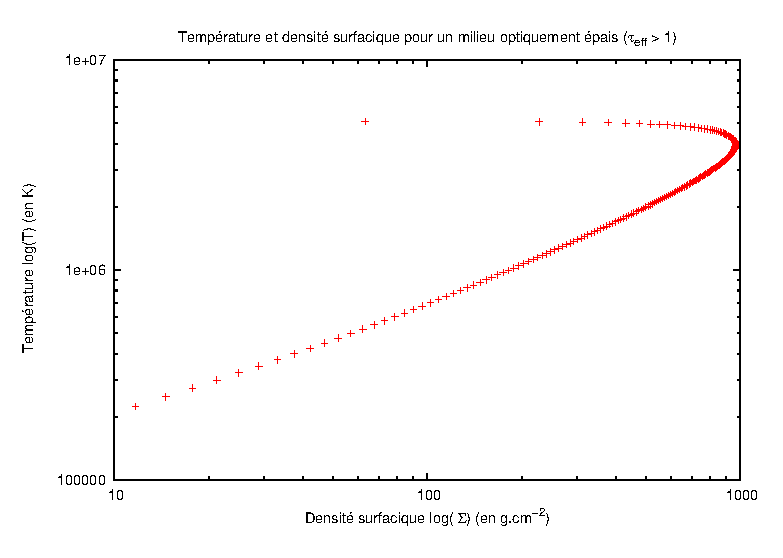
\includegraphics[height=0.3\textwidth]{S_curve_thick.eps} &
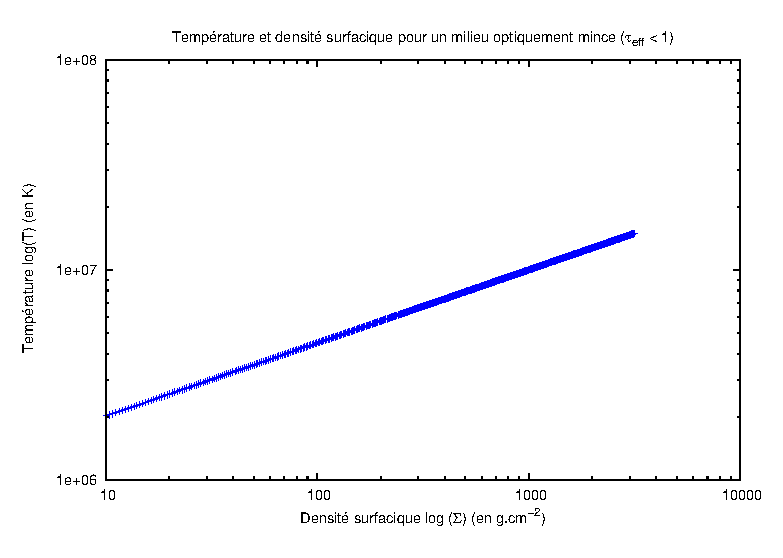
\includegraphics[height=0.3\textwidth]{S_curve_thin.eps} \\
\end{tabular}
  \caption{Cas optiquement épais (gauche) et optiquement mince (droite)}
\label{Fig::}
\end{figure}

La méthode de la dichotomie est une méthode simple et robuste pour trouver les "zéros" d'une fonction mais elle demande un grand nombre de d'itérations. En effet cette méthode converge linéairement.

Le nombre d'itérations par une méthode de dichotomie est donnée par la formule suivante : 
\begin{equation}
n = \frac{log(borne_{sup} - borne_{inf}) + log(\epsilon)}{log(2)} 
\end{equation}

Nous avons donc regardé s' il existait des méthodes qui convergeaient plus rapidement et de manière tout aussi robuste. 

\subsubsection{Méthode de Newton}
La méthode de Newton parfois appelée méthode de Newton-Raphson, décrite dans le \textit{De analysi per aequationes numero terminorum infinitas} en 1669. Cette méthode à l'avantage de converger beaucoup plus rapidement que pour la méthode de la dichotomie (convergence d'ordre 2)

\begin{equation}
x_{k+1} = x_k - \frac{f(x_k)}{f'(x_k)}
\end{equation}

En revanche, cette méthode présente plusieurs inconvénients, tout d'abord, la fonction doit être obligatoirement de classe $C^1$ et le calcul de la dérivée de manière analytique est complexe.


\subsubsection{Méthode de la sécante}

Un des gros inconvénient de la méthode de Newton est d'avoir à calculer la dérivée de la fonction. La méthode de la sécante permet de contourner cet obstacle et ne nécessite pas que la fonction soit de classe $C^1$

\begin{equation}
x_{n+1} = x_n - \frac{x_n - x_{n-1}}{f(x_n) - f(x_{n-1})}
\end{equation}

Cette méthode converge plus rapidement que la méthode de la dichotomie mais moins rapidement que la méthode de Newton (son ordre de convergence est compris entre 0 et 1 \footnote{Pour être plus précis l'ordre de convergence de cette méthode est égale à $\frac{1 + \sqrt{5}}{2}$} qui est le nombre d'or.). Elle permet également de s'affranchir également de la contrainte de l'intervalle de la fonction de la dichotomie. En revanche, cette méthode peut ne pas être robuste si la valeur initiale est trop éloignée de la solution ou s'il existe des racines multiples.

\begin{figure}[htb!]
	\centering
	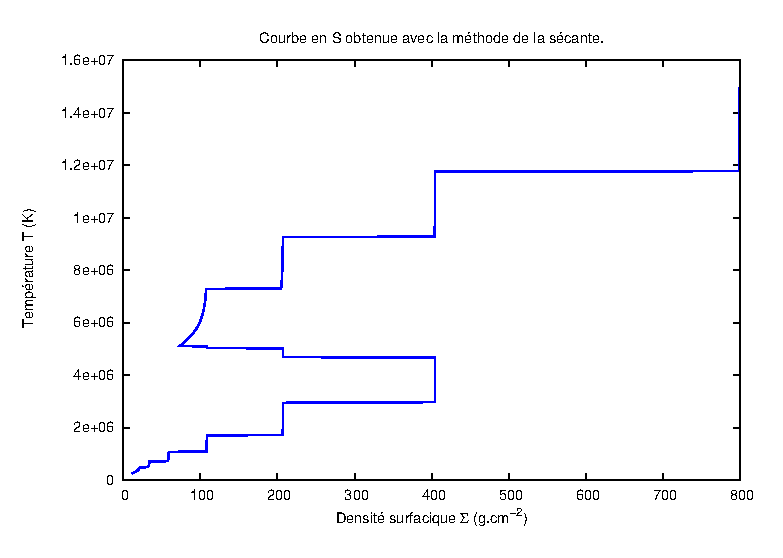
\includegraphics[height=0.7\textwidth]{S_curve_secant.eps}
	\caption{méthode de la sécante}
	\label{Fig::bench}
\end{figure}
%\FloatBarrier


\subsubsection{Méthode de Brent}
La méthode de Brent est une méthode de recherche de "zéros" d'une fonction combinant les méthodes de la dichotomie, de la sécante et l'interpolation quadratique inverse pour en utiliser tous leurs avantages. La méthode de l'interpolation quadratique inverse est une méthode de convergence rapide (ordre 2). Nous pouvons utiliser cette méthode si le dénominateur ne s'annule pas, c'est à dire :
\begin{equation}
f(b) \ne f(a) \text{ et } f(b) \ne f(c) 
\end{equation}
\begin{equation}
x = \frac{(y-f(a)(y-f(b))c}{(f(c)-f(a))(f(c)-f(b))} + \frac{(y-f(b)(y-f(c))a}{(f(a)-f(b))(f(a)-f(c))} +  \frac{(y-f(c)(y-f(a))b}{(f(b)-f(c))(f(b)-f(a))}
\end{equation}
Si cette condition n'est pas réalisée, nous utilisons la méthode de la sécante vue précédemment. Si la méthode de la sécante n'est pas efficace \footnote{C'est à dire.....}, nous utilisons la méthode de la dichotomie.
\\


\subsection{Comparaison des différentes méthodes}

\begin{figure}[htb!]
	\centering
	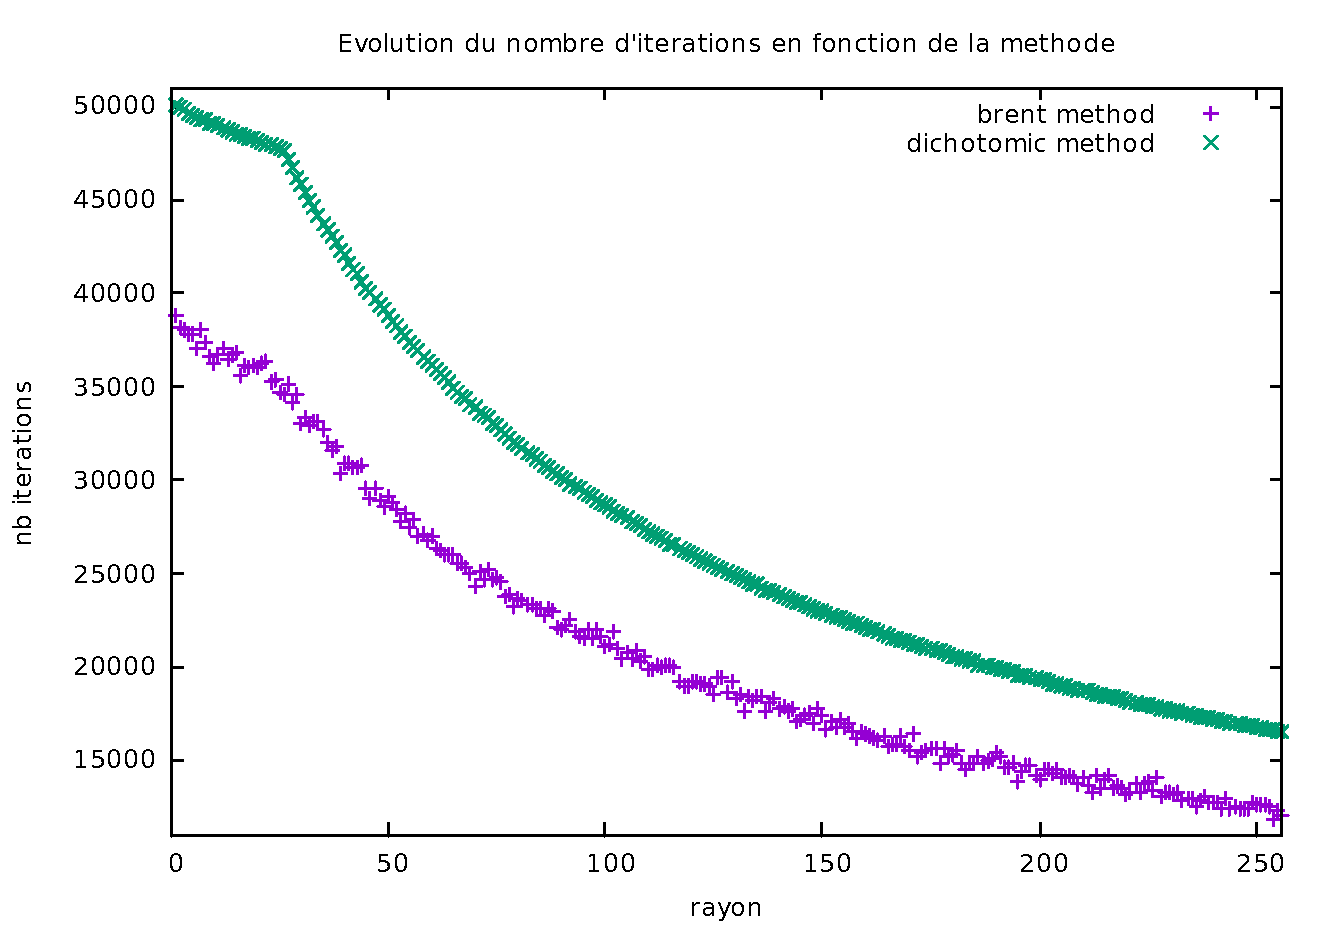
\includegraphics[height=0.5\textwidth]{brent_method3.pdf}
	\caption{Comparaison du nombre d'itérations nécessaire pour converger pour la méthode de la dichotomie et celle de Brent.}
	\label{Fig::bench}
\end{figure}


\subsection{Détermination des points critiques}
Afin de déterminer la propagation de l' instabilité thermique, il faut trouver le point critique où le système devient instable. Au niveau de la courbe en S, ceci a lieu sur la branche inférieure au niveau de la courbure : au-delà de ce point la densité surfacique diminue tandis que la température continue à s' élever. Sur la figure \ref{Fig::stable} la zone d'instabilité est représentée en bleue, les zones de stabilité sont en rouge.

\begin{figure}[htb!]
	\centering
	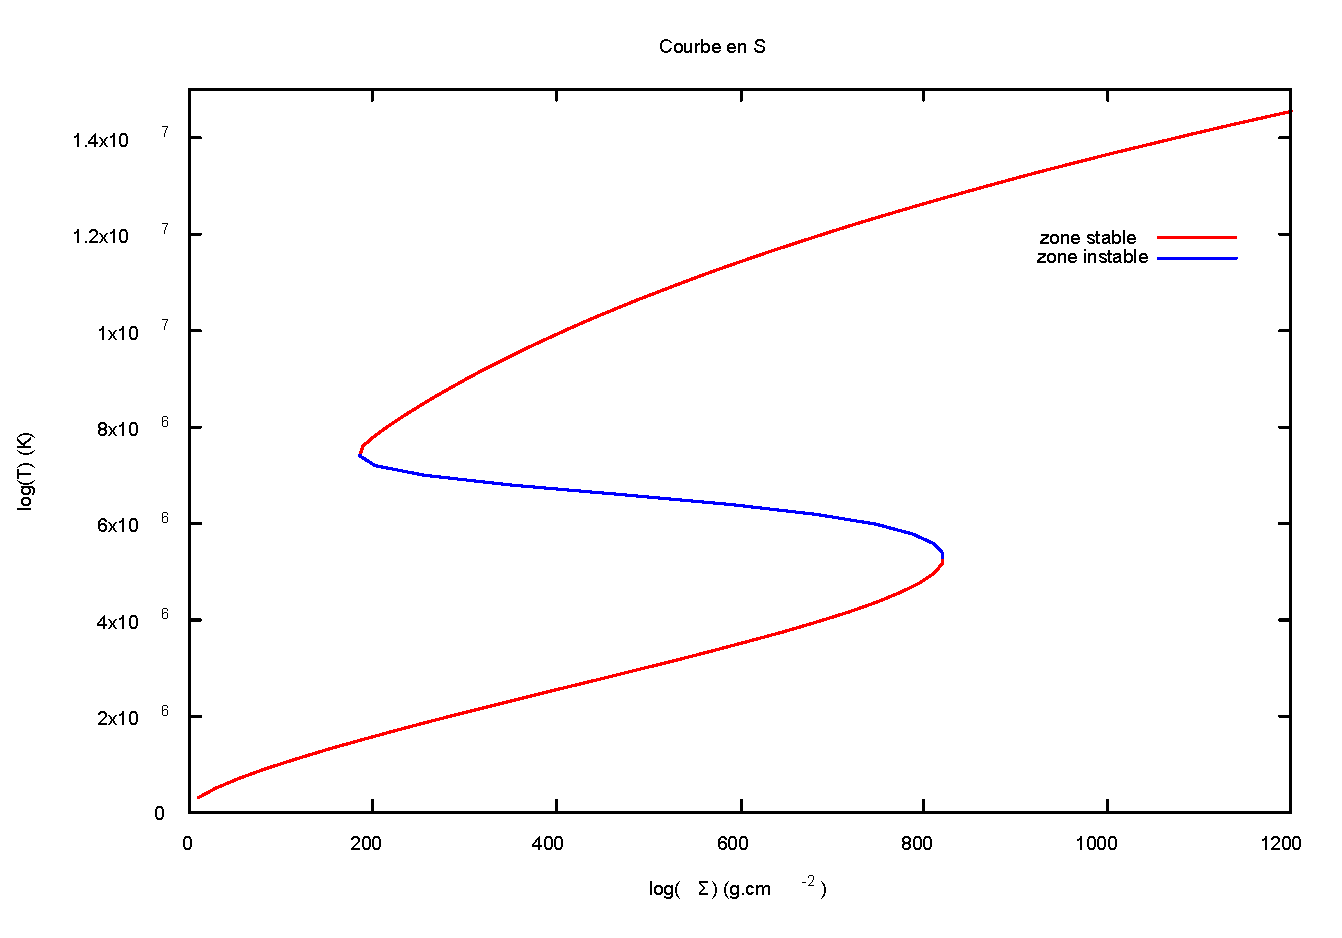
\includegraphics[height=0.7\textwidth]{stable.pdf}
	\caption{Zones stables et instables de la courbe en S}
	\label{Fig::stable}
\end{figure}
%\FloatBarrier

Nous pouvons voir sur ce schéma que la première zone de la courbe en S (la partie la plus basse) correspond à une position stable. Si l'on observe une petite élévation de température (si l'on se place légèrement au-dessus de la courbe), nous arrivons sur une zone ou le terme de refroidissement est supérieur au terme de chauffage, cette partie du disque va donc se refroidir pour retrouver sa position d'équilibre. De même, si l'on observe une petite diminution de température (si l'on se place légèrement en-dessus de la courbe) le terme de chauffage devient supérieur au terme de refroidissement, cette partie du disque va donc se réchauffer jusqu'à retrouver sa position d'équilibre. Il se passe exactement le même phénomène sur la partie haute de la courbe en S (zone III).

En revanche sur la partie centrale de la courbe (zone II), les petites perturbations se retrouvent amplifiées, nous sommes donc sur une section instable.


Pour trouver les coordonnées de ce point critique, nous avons comparé les valeurs de $\Sigma$ (calculé pour un milieu optiquement épais) pour chaque point en augmentant T. Lorsque la variation de la courbe change, c' est-à-dire quand $\Sigma$ cesse d' augmenter et commence à diminuer, nous avons repéré les coordonnées du dernier point pour lequel la densité surfacique croît.  
\\
Dans le code, nous avons nommé "deuxième point critique", le point où a lieu le basculement d'épaisseur optique. Sur les graphes, ce point se situe à l' intersection des deux branches et signale le changement de régime où on a utilisé une approximation de diffusion à une autre approximation où l'on doit prendre en compte les pertes par rayonnement de freinage (le refroidissement par bremsstrahlung).
\\
Pour le repérer, nous avons eu la même approche que pour pour le point d' instabilité trouvé préalablement. Cette fois-ci, nous avons comparé le $\Sigma$ déterminé pour un milieu optiquement épais à celui optiquement mince. Quand le premier devient plus petit que le second, celà signifie que la densité surfacique arrête de décroître et qu' elle commence à augmenter linéairement en fonction de la température. 
\\
%%%%%%%%[courbe en S avec les points légendés + ?evolution en fonction de r ?]

\subsection{Construction de la courbe}

En combinant les points trouvés dans le cas optiquement épais jusqu'au deuxième point critique et les points trouvés dans le cas optiquement mince, nous avons pu assembler les deux parties de la courbe en S.

\begin{figure}[htb!]
	\centering
	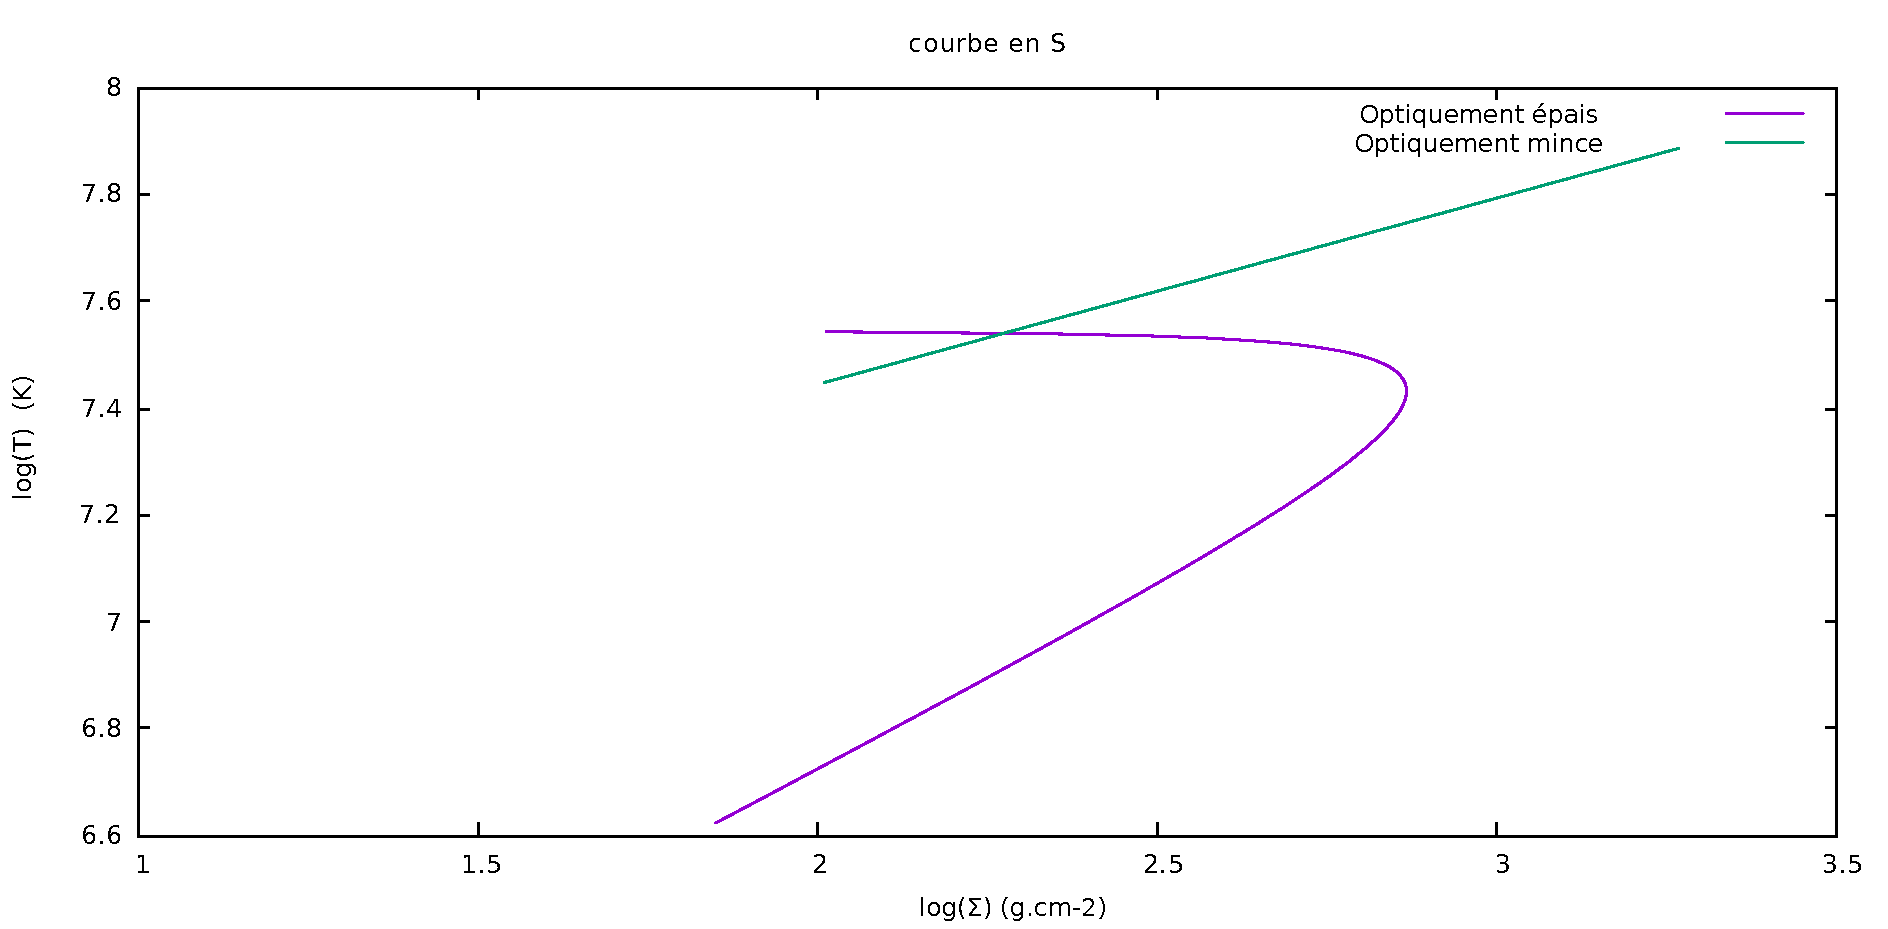
\includegraphics[height=0.5\textwidth]{deux_parties.pdf}
	\caption{Construction de la courbe en S}
	\label{Fig::bench}
\end{figure}


Nous avons donc pour chaque rayon une courbe en S représenté sur le graphe ci-dessous.
\begin{figure}[htb!]
	\centering
	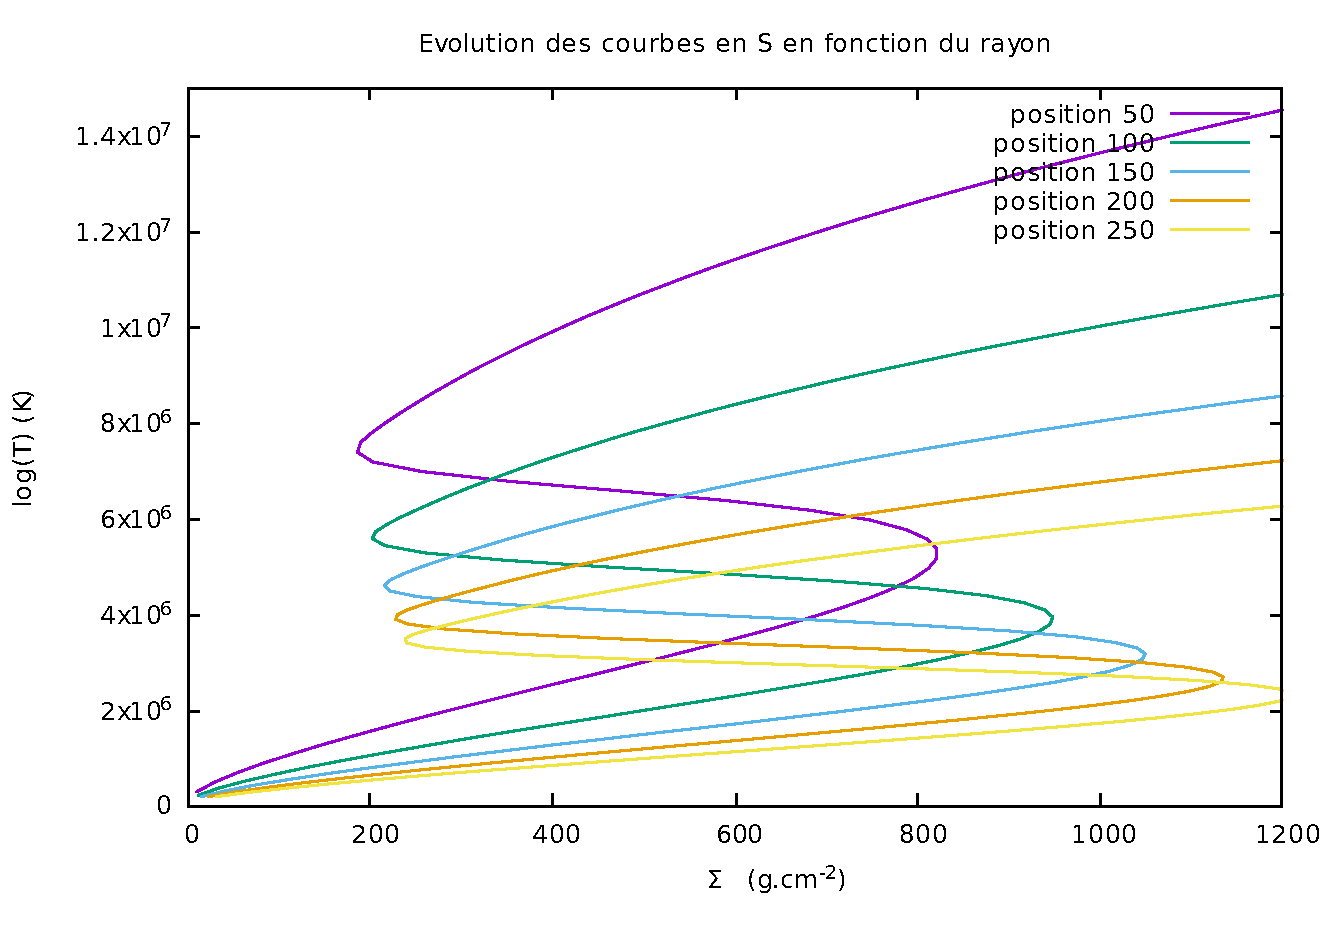
\includegraphics[height=0.7\textwidth]{evolutioncourbes.pdf}
	\caption{Evolution de la courbe en S en fonction de la distance au centre}
	\label{Fig::bench}
\end{figure}



\subsection{Evolution du $\tau_eff$}

D' après nos calculs nous trouvons un $\tau_eff$ aux alentours de 0,06 lors de la transition d'un milieu dit optiquement épais à un milieu optiquement mince. Cette valeur ne correspond pas à la valeur théorique où $\tau_eff$ = 1. 
Celà pose un problème au niveau de la partie d'intégration car notre branche linéaire est translatée par rapport à celle définie par la théorie. 
Cette différence de valeurs peut être expliquée par une erreur au niveau de l’adimensionnement ou bien dans les équations que nous avons utilisées ainsi que peut-être par une faute cachée dans nos paramètres ou nos constantes. 
\\
En fonction du rayon r, les coordonnées dans l' espace {T,$\Sigma$} des points ayant une valeur critique de $\tau_eff$ semblent évoluer de manière à ce que la température diminue et la densité surfacique augmente.
%%%manque d'inspiration  

\begin{figure}[htb!]
	\centering
	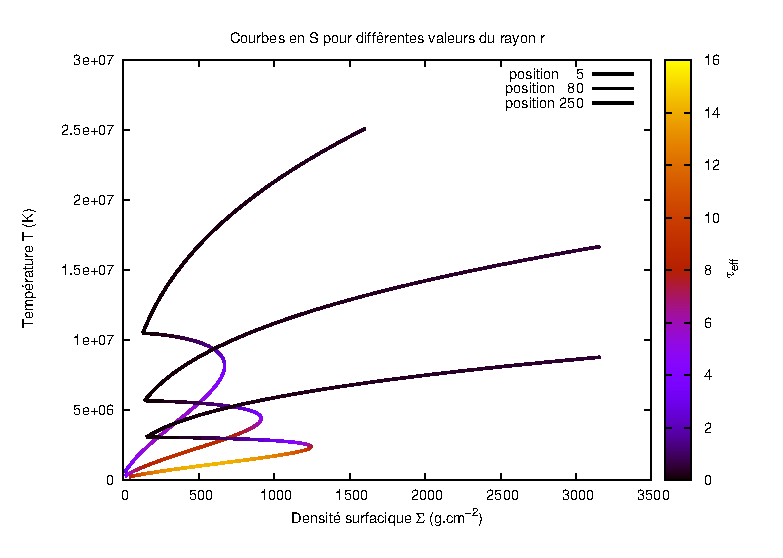
\includegraphics[height=0.7\textwidth]{S_curves_tau.eps}
	\caption{\textit{Evolution de la profondeur optique de la courbe en S pour diffèrents rayons.}  }
	\label{Fig::bench}
\end{figure}

\subsection{Pistes d'améliorations}

\begin{itemize}

\item Calcul direct $Q^+ = Q^-$
\\
Pour définir la température T en fonction de $\Sigma$, nous avons d' abord essayé de simplifier l' égalité $Q^+ = Q^-$ , qui traduit l' équilibre thermique local, en remplaçant tous les termes par T,$\Sigma$ et $\Omega$. Cela donne deux expressions (selon l'opacité du milieu) de fonctions implicites où ces variables sont couplées.
La résolution n' étant pas plus simple qu' avant le changement et afin d' éviter toute erreur induite lors du remplacement des différentes variables impliquées, nous avons préféré de calculer indépendamment chaque variable dans un ordre bien choisi. 
\\

\item Calcul des points critiques par dérivation de la fonction T($\Sigma$)
Comme nous n'avions pas à notre disposition une expression explicite d' allure T = f($\Sigma$), la dérivation des solutions issues d' une série d'équations ne semblait pas l'approche la plus efficace pour trouver le point critique d' instabilité. De plus, en dérivant nous aurions eu un problème au niveau du deuxième point critique qui est un point anguleux.
\end{itemize}

\subsection{Discussion}
Il n'est pas exclu qu'il existe plusieurs racines à l'équation $Q^+ = Q^-$, ce qui voudrait dire que la courbe en S n'est pas unique et plus particulièrement qu'il pourrait exister plusieurs branches dans le cas optiquement mince.

\section{Résolution numérique}

\subsection{Principe de la résolution}

\subsection{Courbe en S}

\subsection{Considérations sur les dérivées}

\begin{equation}
    \frac{\partial u}{\partial t} + v \frac{\partial u}{\partial r} = 0
\end{equation}

\begin{align}
    \frac{\partial u_j}{\partial r} &\approx \frac{u_{j+1} - u_j}{\Delta{r}}
    \frac{\partial u_j}{\partial r} &\approx \frac{u_j - u_{j-1}}{\Delta{r}}
    \frac{\partial u_j}{\partial r} &\approx \frac{u_{j+1} - u_{j-1}}{\Delta{r}}
\end{align}

\begin{equation}
    \frac{\partial \tilde{u}}{\partial t} = - v \frac{\exp(ik\Delta{r}) - \exp(-ik\Delta{r})}{2 \Delta{r}} \tilde{u}
\end{equation}

\begin{align}
    \exp(ik\Delta{r}) &= 1 + ik\Delta{r} + \frac{i^2 k^2 \Delta{r}^2}{2}
    \exp(-ik\Delta{r}) &= 1 - ik\Delta{r} + \frac{i^2 k^2 \Delta{r}^2}{2}
\end{align}

\begin{equation}
    \frac{\partial \tilde{u}}{\partial t} = - v \frac{2ik\Delta{r}}{2\Delta{r}} \tilde{u} = - i k v \tilde{u}
\end{equation}

\begin{equation}
    \tilde{u} = \tilde{u(0)} \exp(-i k v t)
\end{equation}

En fait, nous avons tout simplement :

\begin{equation}
    \frac{\exp(ik\Delta{r}) - \exp(-ik\Delta{r})}{2 \Delta{r}} = \frac{2 i \sin(k\Delta{r})}{2 \Delta{r}} = i k \sinc(k\Delta{r})
\end{equation}

Soit :
\begin{equation}
    \frac{\partial \tilde{u}}{\partial t} = - i k v \sinc(k\Delta{r}) \tilde{u}
\end{equation}

\begin{equation}
    \tilde{u} = \tilde{u(0)} \exp(-i k v \sinc(k \Delta{r}) t)
\end{equation}

\section{Schéma implicite}
\subsection{Intégration de $S$}
\label{subsec:S_integration}
\subsubsection{Linéarisation des équations}
On souhaite intégrer $S^\star$, la densité surfacique adimensionnée. L'équation d'évolution est :
\begin{equation}
  \frac{\partial S^\star}{\partial t^\star} = \frac{1}{x^2}\frac{\partial^2}{\partial x^2}\left(\nu^\star S^\star\right)
\end{equation}
Pour alléger les notations, nous allons ommettre les étoiles dans les développements prochains. L'équation s'écrit alors en passant aux variables discrètes, au temps $t$ et à la case $1<n<n_\textrm{max}$
\begin{equation}
  \label{eq:S_discret_n}
  \frac{S^{t+1}_n - S^t_n}{\Delta t} = \frac{1}{x_n^2}\frac{\nu^t_{n+1}S^{t+1}_{n+1} - 2 \nu^t_nS^{t+1}_n + \nu^t_{n-1}S^{t+1}_{n-1}}{\Delta x^2}
\end{equation}
Pour la case $n = 1$, la quantité $\nu^t_{0}S^{t+1}_{0}$ est supposée nulle et donc: 
\begin{equation}
  \label{eq:S_discret_1}
  \frac{S^{t+1}_1 - S^t_1}{\Delta t} = \frac{1}{x_1^2}\frac{\nu^t_{2}S^{t+1}_{2} - 2 \nu^t_1S^{t+1}_1}{\Delta x^2}
\end{equation}
Pour la case $n = n_\textrm{max} = N$, on a d'après \eqref{eq:nuS_n_is_null}:
\begin{equation}
  \frac{\nu^{t}_{N+1}S^{t+1}_{N+1} - \nu^{t}_NS^{t+1}_N}{\Delta x} = 1
\end{equation}
et donc l'équation \eqref{eq:S_discret_n} s'écrit en $N$:
\begin{equation}
  \label{eq:S_discret_N}
  \frac{S^{t+1}_N - S^t_N}{\Delta t} = \frac{1}{x_N^2}\frac{\Delta x - \nu^{t}_NS^{t+1}_N + \nu^{t}_{N-1}S^{t+1}_{N-1}}{\Delta x^2}
\end{equation}

\subsubsection{Écriture matricielle}
On réécrit \eqref{eq:S_discret_n}, \eqref{eq:S_discret_1} et \eqref{eq:S_discret_N} pour exprimer $S^t$ en fonction de $S^{t+1}$:
\begin{equation}
  \left\lbrace\begin{array}{r l c l c l }
    S^{t}_1 = &
               & &S_1^{t+1}\left(1 + 2\frac{\Delta t}{\Delta x^2}\frac{\nu_1^t}{x_1^2}\right)
               &+& S_{2}^{t+1}\left(-\frac{\Delta t}{\Delta x^2}\frac{\nu_{2}^t}{x_1^2}\right)\\
    S^{t}_n = &S_{n-1}^{t+1}\left(-\frac{\Delta t}{\Delta x^2}\frac{\nu_{n-1}^t}{x_n^2}\right)
               &+& S_n^{t+1}\left(1 + 2\frac{\Delta t}{\Delta x^2}\frac{\nu_n^t}{x_n^2}\right)
               &+& S_{n+1}^{t+1}\left(-\frac{\Delta t}{\Delta x^2}\frac{\nu_{n+1}^t}{x_n^2}\right)\\
    S^{t}_N + \frac{\Delta t}{\Delta x x_N^2} =
               &S^{t+1}_{N-1} \left(-\frac{\Delta t}{\Delta x^2}\frac{\nu_{N-1}^t}{x_N^2}\right)
               &+& S_N^{t+1} \left(1 + \frac{\Delta t}{\Delta x^2}\frac{\nu^t_N}{x_N^2}\right)
               & &
  \end{array}\right.
\end{equation}

Pour simplifier, on notera $A_k = 1 + 2 \frac{\Delta t}{\Delta x^2}\frac{\nu_k^t}{x_k^2}$ et $\Delta = \frac{\Delta t}{\Delta x^2}$
Ce système d'équation s'écrit aussi sous forme matricielle :
\begin{equation}
  \left(S^t\middle) + 
  \middle(\begin{matrix}
    0 \\
    \\
    \\
    \vdots \\
    \\
    \\
    \\
    0 \\
    \frac{\Delta t}{\Delta x}\frac{1}{x_N^2}
  \end{matrix}\middle)
  =
  \begin{pmatrix}
A_1                            & -\Delta\frac{\nu_{2}^t}{x_1^2} &  & & & & 0\\
-\Delta \frac{\nu_{1}^t}{x_2^2} & A_2                           & -\Delta\frac{\nu_{3}^t}{x_2^2} & & & &\\
    &        & \ddots                          &  & & & &\\
    &        & -\Delta \frac{\nu_{k-1}^t}{x_k^2} & A_k    & -\Delta \frac{\nu_{k+1}^t}{x_k^2} & &\\
    &        &                                 & & \ddots                          & & \\
    & & & & -\Delta \frac{\nu_{N-2}^t}{x_{N-1}^2} & A_{N-1} & -\Delta \frac{\nu_{N}^t}{x_{N-1}^2}\\
    0 & & & & & -\Delta \frac{\nu_{N-1}^t}{x_N^2} & 1 + \Delta \frac{\nu_N^t}{x_N^2}
  \end{pmatrix} \middle(S^{t+1}\right)
\end{equation}
Qui s'écrit aussi :
\begin{equation}
  AS^{t+1} = S^t + X 
\end{equation}

\subsection{Intégration de $T$}
\label{subsec:integration_T}

Si on est dans le cas optiquement mince (ou bien négligeons terme advection ??), $T$ est régit par l'équation :
\begin{equation}
  C_v^\star \frac{\partial T^\star}{\partial t^\star} = 3v_0^2\nu^\star \Omega^\star{}^2 - \frac{F_z^\star x}{S^\star}
\end{equation}

\subsubsection{Linéarisation}
On va écrire l'équation linéarisée pour $T$. Une fois encore, nous allons ommettre les ${}^\star$ pour alléger les notations.

On note $f(T, S) = \frac{\partial T}{\partial t}(T, S)$ et $f_1(T, S) = \frac{\partial f}{\partial T}$
\begin{equation}
  \label{eq:T_devpmt_lin_2e_ordre} 
  \frac{T(t+\Delta t) - T(t)}{\Delta t} = f(T(t), S(t)) + \Delta Tf_1 + \Delta S\frac{\partial f}{\partial S}
\end{equation}
Comme $\tau_\textrm{therm} \ll \tau_\textrm{dyn}$, on va pouvoir négliger $\frac{\Delta S}{\tau_\textrm{therm}}$ devant $\frac{\Delta T}{\tau_\textrm{therm}}$. L'équation \eqref{eq:T_devpmt_lin_2e_ordre} s'écrit alors :
\begin{equation}
  \frac{T(t+\Delta t) - T(t)}{\Delta t} = f(T, S) + \Delta T f_1 = f(T, S) + \Delta t \underbrace{\frac{\Delta T}{\Delta t}}_{f} f_1
\end{equation}
Finalement, on obtient avec les écritures discrètes:
\begin{equation}
  T^{t+1}_n = T^{t}_n + \Delta t f^t_n \left(1 + \Delta t {f_1^t}_n\right)
\end{equation}

\subsubsection{Approximation de $f_1$}
Pour approximer $f_1^t$, on utilisera :
\begin{equation}
  {f_1^t}_n = \frac{f(T_n^t+\Delta T_n^t) - f(T_n^t)}{\Delta T_n^t}, \quad \Delta T_n^t = \alpha T_n^t,\ \alpha \ll 1
\end{equation}
%%% Local Variables:
%%% mode: latex
%%% TeX-master: "rapport"
%%% End:


\include{integration}

\section{dérivation partielle  de $S^{\star}$ et $T^{\star}$}

\subsection{Méthode de dérivation}

Pour intégrer les équation de $S$ et $T$ (\eqref{eq:difS} et \eqref{eq:difT}), on choisit de réaliser une dérivée amont. Dans le cas présent, il s'agit d'une dérivée dans le sens croissant des indices du tableau. Ainsi pour calculer la dérivé partielle de $S^{\star}$ en $x$ à la case $i$ on calculera :

\begin{equation}
  \left. \frac{\partial S^{\star}}{\partial x} \right|_i = \frac{S^{\star}(i+1)-S^{\star}(i)}{\delta x} 
\end{equation}

Et pour calculer la dérivée seconde de $S^{\star}$ en $x$ à la case $i$ :

\begin{equation}
  \left. \frac{\partial^2 S^{\star}}{\partial x^2}\right|_i=\frac{S^{\star}(i+1)-2\ S^{\star}(i) +S^{\star}(i-1)}{\delta x^2} 
\end{equation}

Cependant, on constate qu'avec cette méthode il nous faut connaître la valeur de la case $i+1$, case inexistante dans le cas $i=i_{max}$.

\subsection{Condition au bords de $\nu^{\star}S^{\star}$}

\subsubsection{Dérivée partielle première}

Dans l'équation différentielle sur $v^{\star}$ \eqref{eq:difv} on doit connaître $\frac{\partial \nu^{\star} S^{\star}}{\partial x}$ en $i=i_{max}$.
On fait l'hypothèse qu'en $r_{max}$ le taux d'accrétion est $\dot{M}_0$. Dés lors par \eqref{eq:Mdotstar} on a $(\dot{M}^{\star}_0=)1 = -(x S^{\star}v^{\star})$ et par \eqref{eq:difv} il vient :

\begin{equation}
  \label{eq:nuS_n_is_null}
  \left. \frac{\partial (\nu^{\star} S^{\star})}{\partial x}\right|_{i=i_{max}}=1
\end{equation}


\subsubsection{dérivée partielle seconde}
Afin de calculer $\frac{\partial^2(\nu^{\star} S^{\star})} {\partial x^2}$ en $i=i_{max}$ il nous faut connaître les valeurs hypothétiques de $(\nu^{\star} S^{\star})(i=i_{max}+1)$ que l'on va obtenir à partir des valeurs des dérivées premières. On a donc :

\begin{eqnarray}
  \left. \frac{\partial (\nu^{\star}S^{\star})}{\partial x} \right|_{i_{max}} = 1 = \frac{(\nu^{\star} S^{\star})(i_{max}+1)-(\nu^{\star}S^{\star})(i_{max})}{\delta x} 
\end{eqnarray}

Dès lors on a : 
\begin{equation}
( \nu^{\star} S^{\star})(i_{max}+1) = \delta x + (\nu^{\star}S^{\star})(i_{max}) 
\end{equation}

Il vient donc :
\begin{eqnarray}
 \left. \frac{\partial^2 (\nu^{\star} S^{\star})}{\partial x^2}\right|_{i=i_{max}} &=& \frac{(\nu^{\star} S^{\star})(i_{max}+1) - 2\ (\nu^{\star} S^{\star})(i_{max}) + (\nu^{\star} S^{\star})(i_{max}-1)}{\delta x^2}\\
 \left. \frac{\partial^2 (\nu^{\star} S^{\star})}{\partial x^2}\right|_{i=i_{max}} &=& \frac{\delta x - (\nu^{\star} S^{\star})(i_{max}) + (\nu^{\star} S^{\star})(i_{max}-1)}{\delta x^2}
\end{eqnarray}

\subsection{Conditions aux bords de $S^{\star}$}
On cherche les conditions aux bords de $\frac{\partial S^{\star}}{\partial t^{\star}}$, pour cela on utilise l'équation \eqref{eq:difS}. Dès lors on a directement :

\begin{eqnarray}
  \left. \frac{\partial S^{\star}}{\partial t^{\star}} \right|_{i=i_{max}}&= \frac{1}{(x(i_{max}))^2} \left. \frac{\partial^2 (\nu^{\star} S^{\star})}{\partial x^2}\right|_{i=i_{max}} &= \frac{1}{(x(i_{max}))^2} \frac{\delta x - (\nu^{\star} S^{\star})(i_{max}) + (\nu^{\star} S^{\star})(i_{max}-1)}{\delta x^2}
\end{eqnarray}


\subsection{Condition aux bords de $S^{\star}/x$}

Dans l'équation \eqref{eq:difT} il est nécessaire de connaître les valeurs $\frac{\partial}{\partial x}\left(\frac{S^{\star}}{x}\right)$ en chacun des points du disque, donc en $i=i_{max}$. 

On a fais comme hypothèse que la partie du disque la plus éloigné du trou noire ($i_{max}$) reste toujours stable. Par conséquent, $Q_{adv}$ est toujours négligeable devant $Q^+$ et $Q^-$. On a donc 

\begin{equation}
Q_{adv}=\frac{\mathcal{R} T_0}{\mu} \frac{4-3\beta}{\beta} \frac{T^\star}{S^\star} \times
        \left( \frac{\partial S^\star}{\partial t^\star} + v^\star \frac{\partial}{\partial x} \left(\frac{S^\star}{x}\right) \right) -
        \frac{C_v^\star v^\star}{x} \frac{\partial T^\star}{\partial x}=0
\end{equation}

Or d'après nos hypothèse la température ne varie pas en $i_{max}$ donc $\frac{\partial T^\star}{\partial x} =0$ dés lors on a :


\begin{equation}
  \frac{\partial S^{\star}}{\partial t^{\star}} + v^{\star} \frac{\partial}{\partial x} \left(\frac{S^{\star}}{x}\right)=0
\end{equation}

Donc avec \eqref{eq:difT}

\begin{equation}
  \frac{\partial}{\partial x} \left(\frac{S^{\star}}{x}\right) = -\frac{1}{x^2\ v^{\star}} \frac{\partial^2 (\nu^{\star} S^{\star})}{\partial x^2}
\end{equation}

dés lors on a :

\begin{equation}
\left. \frac{\partial}{\partial x} \left(\frac{S^{\star}}{x}\right) \right|_{i_{max}} = \left. -\frac{1}{x^2\ v^{\star}} \frac{\partial^2 (\nu^{\star} S^{\star})}{\partial x^2} \right|_{i_{max}} = \frac{1}{(x^2\ v^{\star})(i_{max})} \frac{\delta x - (\nu^{\star} S^{\star})(i_{max}) + (\nu^{\star} S^{\star})(i_{max}-1)}{\delta x^2}
\end{equation}




%\section{integration de $S^{\star}$ et $T^{\star}$ (mauvaise facons) et condition au bord}

\subsection{Méthode d'intégration}

Pour intégrer les équation de S et T (\eqref{eq:difS} et \eqref{eq:difT}), étant donné que ce ne sont pas des équation de transport, nous avons le choix du sens d'intégration. Afin de gagner en précision, pour la dérivée en un point on fera la moyenne des dérivé a droite et a gauche. Ainsi pour calculer la dérivé partielle de $S^{\star}$ en x a la case $i$ on calculera :

\begin{equation}
  \left. \frac{\partial S^{\star}}{\partial x} \right|_i = \frac{S^{\star}(i+1)-S^{\star}(i-1)}{2\delta x} \label{eq:dif_ordre1}
\end{equation}

Et pour calculer la dérivée seconde de $S^{\star}$ par en x a la case $i$ :

\begin{equation}
  \left. \frac{\partial^2 S^{\star}}{\partial x^2}\right|_i=\frac{S^{\star}(i+1)-2\ S^{\star}(i) +S^{\star}(i-1)}{\delta x^2} \label{eq:dif_ordre2}
\end{equation}

Cependant, on constate qu'avec cette méthode il est nécessaire de connaitre la valeur des cases voisines, or la première ($i=1$) et la dernière ($i=i_{max}$) n'ont pas de voisin de part et d'autre, il nous faut donc déterminer des condition au bord.


\subsection{Condition au bords de $\nu^{\star}S^{\star}$}

\subsubsection{dérivée partielle première}

Dans l'équation différentielle sur $v^{\star}$ \eqref{eq:difv} on doit connaitre $\frac{\partial \nu^{\star} S^{\star}}{\partial x}$ en $i=1$ et $i=i_{max}$.

\paragraph{$i=1$}
Dans ce projet on fais l'hypothèse que en $r_{min}$ toute la matière est accréter par le trou noir donc $\Sigma(r_{min})=0$ de pars l'adimensionnement que l'on a pris il vient $S^{\star}(i=1)=0$ dés lors par l'équation \eqref{eq:difv} on a

\begin{equation}
  \left. \frac{\partial (\nu^{\star} S^{\star})}{\partial x}\right|_{i=1}=0\label{eq:dif_nuS_i1}
\end{equation}

\paragraph{$i=i_{max}$}
On fais l'hypothèse que en $r_{max}$ le taux d'accrétion est $\dot{M}_0$ dés lors par \eqref{eq:Mdotstar} on a $(\dot{M}^{\star}_0=)1 = -(x S^{\star}v^{\star})$ et par \eqref{eq:difv} il vient :

\begin{equation}
  \left. \frac{\partial (\nu^{\star} S^{\star})}{\partial x}\right|_{i=i_{max}}=1\label{eq:dif_nuS_imax}
\end{equation}

\subsubsection{dérivée partielle seconde}
Afin de calculé $\frac{\partial^2(\nu^{\star} S^{\star})} {\partial x^2}$ en $i=1$ et $i=i_{max}$ il nous faut connaitre les valeur hypothétique de $(\nu^{\star} S^{\star})(i=1-1)$ et $(\nu^{\star} S^{\star})(i=i_{max}+1)$ que l'on va obtenir a partir des valeurs des dérivée première.

\paragraph{i=1}
On a d'après \eqref{eq:dif_ordre1} et \eqref{eq:dif_nuS_i1} :
\begin{equation}
  \left. \frac{\partial (\nu^{\star} S^{\star})}{\partial x}\right|_{i=1}=0=\frac{ (\nu^{\star} S^{\star})(1+1) - (\nu^{\star} S^{\star})(1-1)}{2\delta x}
\end{equation}

dès lors
\begin{equation}
  (\nu^{\star} S^{\star})(1-1)=(\nu^{\star} S^{\star})(1+1)
\end{equation}

On en déduit donc la condition au bord :

\begin{eqnarray}
  \left. \frac{\partial^2 (\nu^{\star} S^{\star})}{\partial x^2}\right|_{i=1} &=& \frac{(\nu^{\star} S^{\star})(1+1) -2\ \overbrace{(\nu^{\star} S^{\star})(1)}^{=0}+ (\nu^{\star} S^{\star})(1-1)}{\delta x ^2} \\
  \left. \frac{\partial^2 (\nu^{\star} S^{\star})}{\partial x^2}\right|_{i=1} &=& \frac{2\ (\nu^{\star} S^{\star})(2)}{\delta x ^2}
\end{eqnarray}

\paragraph{$i=i_{max}$}
De même que pour $i=1$ on utilise la valeur de la dérivée première pour calculer $(\nu^{\star} S^{\star})(i_{max}+1)$, on obtient :
\begin{equation}
  (\nu^{\star} S^{\star})(i_{max}+1)=2\delta x + (\nu^{\star} S^{\star})(i_{max}-1)
\end{equation}

Il vient donc 
\begin{eqnarray}
  \left. \frac{\partial^2 (\nu^{\star} S^{\star})}{\partial x^2}\right|_{i=i_{max}} &=& \frac{(\nu^{\star} S^{\star})(i_{max}+1) - 2\ (\nu^{\star} S^{\star})(i_{max}) + (\nu^{\star} S^{\star})(i_{max}-1)}{\delta x^2}\\
  \left. \frac{\partial^2 (\nu^{\star} S^{\star})}{\partial x^2}\right|_{i=i_{max}} &=& 2\ \frac{\delta x + (\nu^{\star} S^{\star})(i_{max}-1)- (\nu^{\star} S^{\star})(i_{max})}{\delta x^2}
\end{eqnarray}

\subsection{conditions aux bords de $S^{\star}$}
On cherche les condition au bords de $\frac{\partial S^{\star}}{\partial t^{\star}}$, pour cela on utilise l'équation \eqref{eq:difS}. Dès lors on a directement :

\begin{eqnarray}
  \left. \frac{\partial S^{\star}}{\partial t^{\star}} \right|_{i=1} &= \frac{1}{(x(1))^2} \left. \frac{\partial^2 (\nu^{\star} S^{\star})}{\partial x^2}\right|_{i=1} &= \frac{1}{(x(1))^2} \frac{2\ (\nu^{\star} S^{\star})(2)}{\delta x ^2}\\
  \left. \frac{\partial S^{\star}}{\partial t^{\star}} \right|_{i=i_{max}}&= \frac{1}{(x(i_{max}))^2} \left. \frac{\partial^2 (\nu^{\star} S^{\star})}{\partial x^2}\right|_{i=i_{max}} &= \frac{2}{(x(i_{max}))^2} \frac{\delta x + (\nu^{\star} S^{\star})(i_{max}-1)- (\nu^{\star} S^{\star})(i_{max})}{\delta x^2}
\end{eqnarray}

\subsection{condition aux bords de $S^{\star}/x$}

Dans l'équation \eqref{eq:difT} il est nécessaire de connaitre les valeur $\frac{\partial}{\partial x}\left(\frac{S^{\star}}{x}\right)$ en chacun des point du disque, donc a chacune des extrémités. 

%FIXME
On a : (je ne sais plus l'argument !!!)
\begin{equation}
  \frac{\partial S^{\star}}{\partial t^{\star}} + v^{\star} \frac{\partial}{\partial x} \left(\frac{S^{\star}}{x}\right)=0
\end{equation}

Donc avec \eqref{eq:difT}

\begin{equation}
  \frac{\partial}{\partial x} \left(\frac{S^{\star}}{x}\right) = -\frac{1}{x^2\ v^{\star}} \frac{\partial^2 (\nu^{\star} S^{\star})}{\partial x^2}
\end{equation}

On en déduit donc :

\begin{eqnarray}
  \left. \frac{\partial}{\partial x} \left(\frac{S^{\star}}{x}\right) \right|_{i=1 }&=& - \frac{1}{(x^2\ v^{\star})(1)} \frac{2\ (\nu^{\star} S^{\star})(2)}{\delta x ^2} \\
  \left. \frac{\partial}{\partial x} \left(\frac{S^{\star}}{x}\right) \right|_{i=i_{max}} &=& - \frac{2}{(x^2\ v^{\star})(i_{max})} \frac{\delta x + (\nu^{\star} S^{\star})(i_{max}-1)- (\nu^{\star} S^{\star})(i_{max})}{\delta x^2}
\end{eqnarray}


\section{Résultats et interprétations}

Nous avons fait tourner cette simulation pour une durée totale physique de 26141802 secondes, soit l'équivalent de 302.6 jours. 
Les solutions pour chaque $r$ de la branche supérieure déterminé par dichotomie ne sont pas les branches atteintes dans la simulations. Nous pouvons voir sur la figure (\ref{fig:tau.png}) en rouge la branche déterminer par dichotomie correspondant à $\tau_{ff} = 0.06 $ et en blanc celle correspondant à la valeur théorique $\tau_{ff} = 1$. Les possibles raisons de cet écarts sont dévelopés partie (\ref{sec::pistes}). La simulation est bien en accord avec le passage d'un disque optiquement épais à un disque optiquement mince.  

\begin{figure}
  \begin{center}
    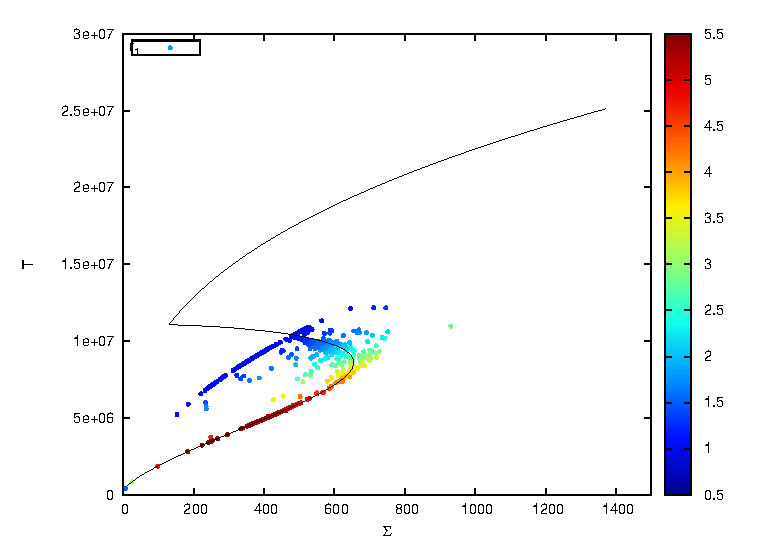
\includegraphics[]{c1.eps}
  \end{center}
  \caption{$T=f(\Sigma)$, $\Delta t = 26141802 s$ (durée de la simulation) pour $r_{1}$. Le gradiant de couleur représente les valeurs de $\tau_{ff}$}
  \label{fig:c1.eps}
\end{figure} 

\begin{figure}
  \begin{center}
    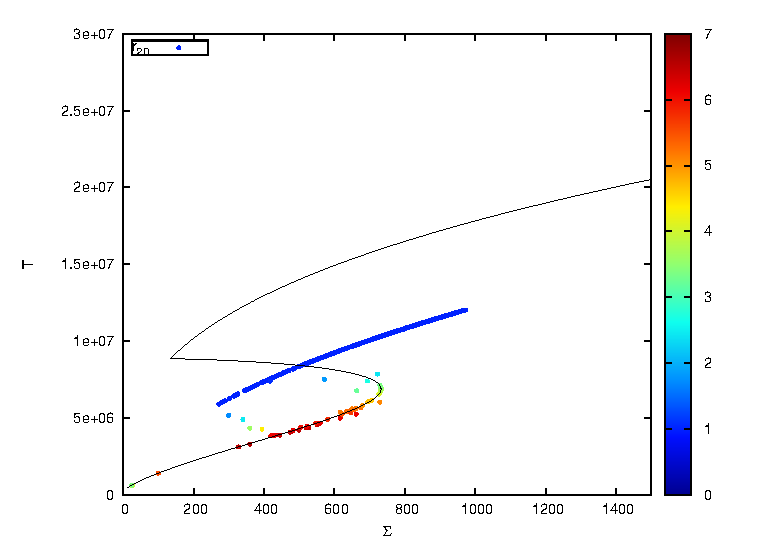
\includegraphics[]{c20.eps}
  \end{center}
  \caption{$T=f(\Sigma)$, $\Delta t = 26141802 s$ (durée de la simulation) pour $r_{20}$. Le gradiant de couleur représente les valeurs de $\tau_{ff}$}
  \label{fig:c20.eps}
\end{figure}


\begin{figure}
  \begin{center}
    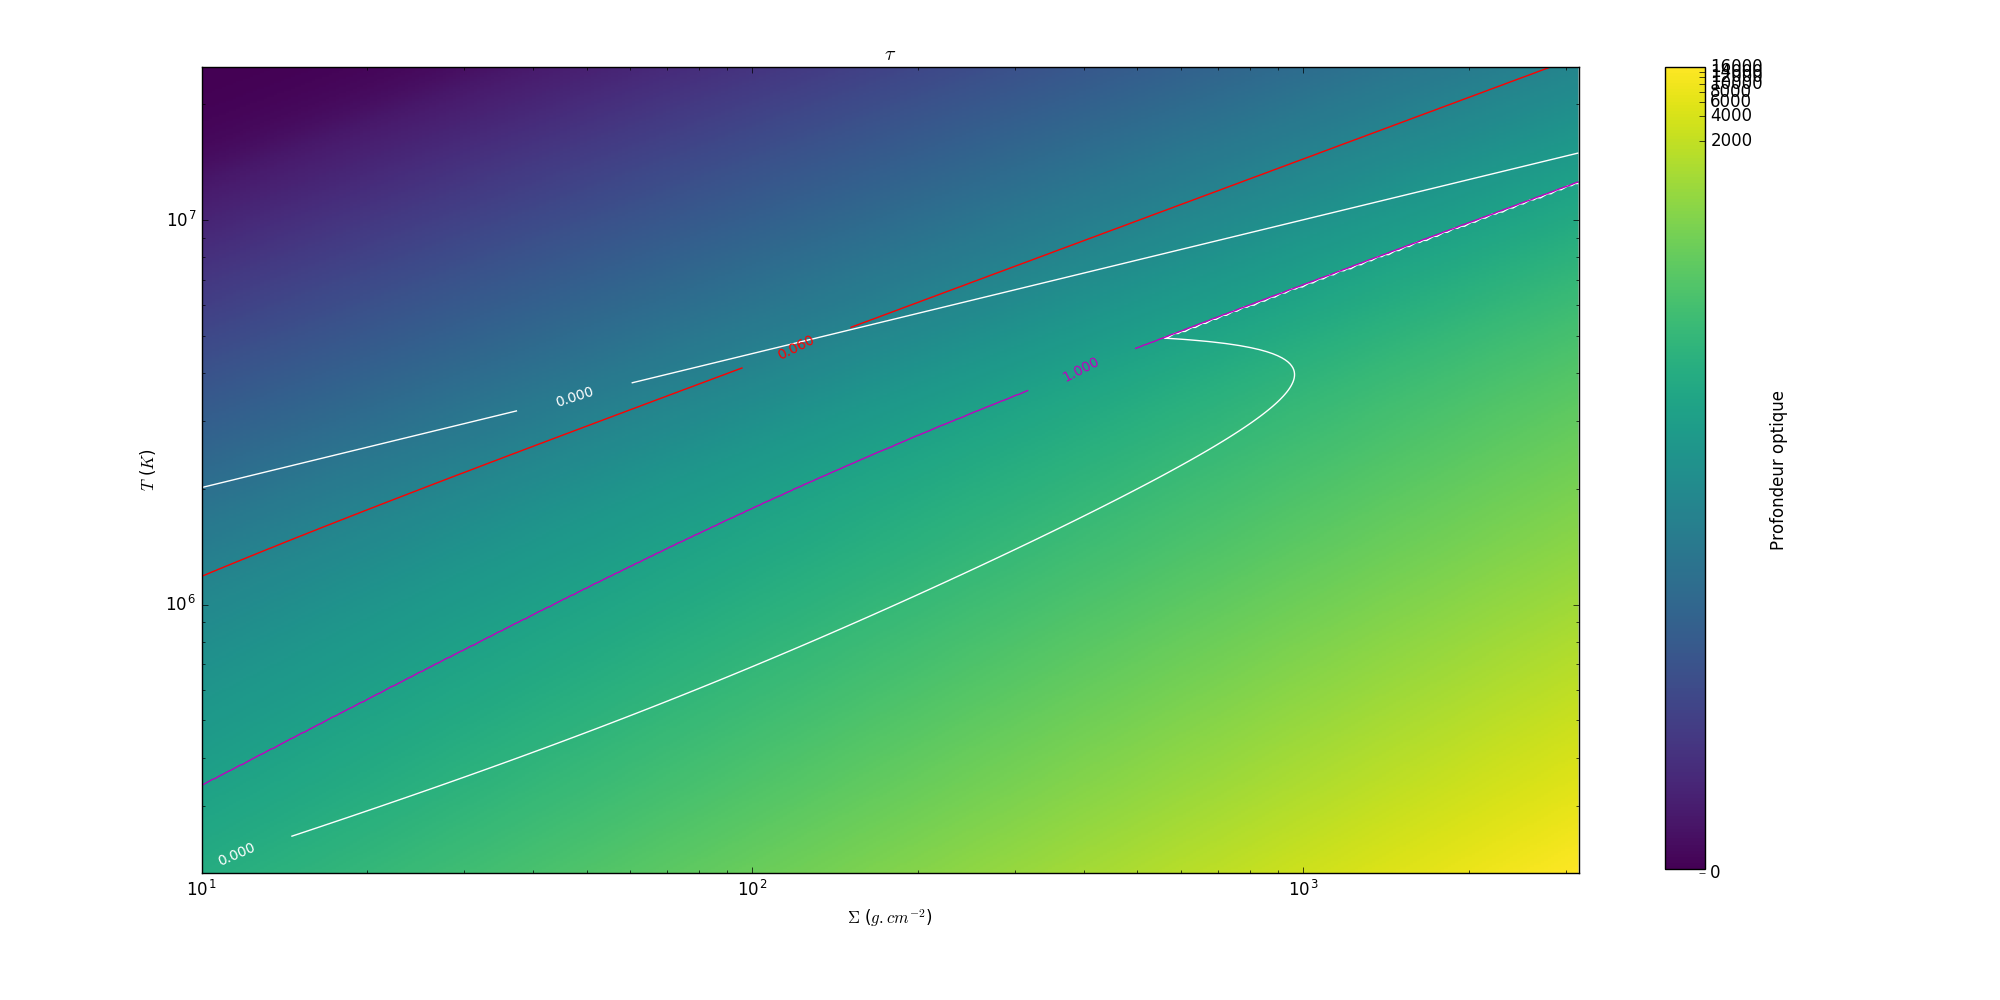
\includegraphics[scale=0.36]{tau.png}
  \end{center}
  \caption{..}
  \label{fig:tau.png}
\end{figure} 



\section*{Conclusion}
\addcontentsline{toc}{section}{Conclusion}



\appendix

\makeatletter
\def\@seccntformat#1{Annexe~\csname the#1\endcsname:\quad}
\makeatother

\section{Calculs sur l’adimensionnement}

\begin{align}
    \left\{
        \begin{aligned}
            \partial T &= \partial T^{\star} × T_0 \\
            \partial t &= \frac{\partial t^{\star}}{\Omega_{max}}
        \end{aligned}
    \right.
\end{align}

\begin{equation}
    T_0 \Omega_\mathrm{max} C_v \frac{\partial T^{\star}}{\partial t^{\star}} =
    3 \Omega^2 \nu^\star \Omega_\mathrm{max} r_s^2 − \frac{2 F_z x}{S} +
    \frac{R}{\mu} \left(\frac{4−3\beta}{\beta}\right) \frac{T^\star T_0 x}{S}
    \left( \frac{\partial S}{\partial t^\star} \frac{\Omega_\mathrm{max}}{x} + v \frac{\partial}{\partial x} \left(\frac{S}{x}\right) \frac{1}{2 r^½ r_s^½}  \right) –
    C_v v \frac{\partial T^\star}{\partial x} \frac{T_0}{2 r^½ r_s^½}
\end{equation}

\begin{equation}
    T_0 C_v \frac{\partial T^{\star}}{\partial t^{\star}} =
    3 \Omega^2 \nu^\star r_s^2 − \frac{2 F_z x}{S \Omega_\mathrm{max}} +
    \frac{R}{\mu} \left(\frac{4−3\beta}{\beta}\right) \frac{T^\star T_0 x}{S}
    \left( \frac{\partial S}{\partial t^\star} \frac{1}{x} + \frac{v}{\Omega_\mathrm{max}} \frac{\partial}{\partial x} \left(\frac{S}{x}\right) \frac{1}{2 r^½ r_s^½}  \right) –
    \frac{C_v v}{\Omega_\mathrm{max}} \frac{\partial T^\star}{\partial x} \frac{T_0}{2 r^½ r_s^½}
\end{equation}

\begin{equation}
    T_0 C_v \frac{\partial T^{\star}}{\partial t^{\star}} =
    3 \Omega^2 \nu^\star r_s^2 − \frac{2 F_z x}{S \Omega_\mathrm{max}} +
    \frac{R}{\mu} \left(\frac{4−3\beta}{\beta}\right) \frac{T^\star T_0 x}{S}
    \left( \frac{\partial S}{\partial t^\star} \frac{1}{x} − \frac{r_s}{S x} \frac{\partial}{\partial x} \left(\nu^\star S\right) \frac{\partial}{\partial x} \left(\frac{S}{x}\right) \frac{1}{r^½ r_s^½}  \right) –
    \frac{C_v r_s}{S x} \frac{\partial}{\partial x} \left(\nu^\star S\right) \frac{\partial T^\star}{\partial x} \frac{T_0}{r^½ r_s^½}
\end{equation}

\begin{equation}
    T_0 C_v \frac{\partial T^{\star}}{\partial t^{\star}} =
    3 \Omega^2 \nu^\star r_s^2 − \frac{2 F_z x}{S \Omega_\mathrm{max}} +
    \frac{R}{\mu} \left(\frac{4−3\beta}{\beta}\right) \frac{T^\star T_0 x}{S}
    \left( \frac{\partial S}{\partial t^\star} \frac{1}{x} − \frac{1}{S x^2} \frac{\partial}{\partial x} \left(\nu^\star S\right) \frac{\partial}{\partial x} \left(\frac{S}{x}\right) \right) –
    \frac{C_v T_0}{S x^2} \frac{\partial}{\partial x} \left(\nu^\star S\right) \frac{\partial T^\star}{\partial x}
\end{equation}

On regarde le premier terme :
\begin{equation}
    3 \Omega^2 \nu^\star r_s^2 = 3 \frac{\Omega^2}{\Omega_\mathrm{max}^2} \frac{G M \nu^\star}{27 r_s} = {\Omega^\star}^2 \frac{G M \nu^\star}{3 r_\mathrm{min}}
\end{equation}

Soit :
\begin{equation}
    T_0 C_v \frac{\partial T^{\star}}{\partial t^{\star}} =
    {\Omega^\star}^2 \frac{G M \nu^\star}{3 r_\mathrm{min}} − \frac{2 F_z x}{S \Omega_\mathrm{max}} +
    \frac{R}{\mu} \left(\frac{4−3\beta}{\beta}\right) \frac{T^\star T_0 x}{S}
    \left( \frac{\partial S}{\partial t^\star} \frac{1}{x} − \frac{1}{S x^2} \frac{\partial}{\partial x} \left(\nu^\star S\right) \frac{\partial}{\partial x} \left(\frac{S}{x}\right) \right) –
    \frac{C_v T_0}{S x^2} \frac{\partial}{\partial x} \left(\nu^\star S\right) \frac{\partial T^\star}{\partial x}
\end{equation}

\begin{equation}
    T_0 C_v \frac{\partial T^{\star}}{\partial t^{\star}} =
    {\Omega^\star}^2 \frac{G M \nu^\star}{3 r_\mathrm{min}} − \frac{2 F_z x}{S^\star \Omega_\mathrm{max}} +
    \frac{R}{\mu} \left(\frac{4−3\beta}{\beta}\right) \frac{T^\star T_0 x}{S^\star}
    \left( \frac{\partial S^\star}{\partial t^\star} \frac{1}{x} − \frac{1}{S^\star x^2} \frac{\partial}{\partial x} \left(\nu^\star S^\star\right) \frac{\partial}{\partial x} \left(\frac{S^\star}{x}\right) \right) –
    \frac{C_v T_0}{S^\star x^2} \frac{\partial}{\partial x} \left(\nu^\star S^\star\right) \frac{\partial T^\star}{\partial x}
\end{equation}

Par rapport aux photos, je simplifie un $x$ en plus dans le terme central (si ça vous va sous cette forme, je propose de le simplifier plus tôt) :

\begin{equation}
    T_0 C_v \frac{\partial T^{\star}}{\partial t^{\star}} =
    {\Omega^\star}^2 \frac{G M \nu^\star}{3 r_\mathrm{min}} − \frac{2 F_z x}{S^\star \Omega_\mathrm{max}} +
    \frac{R}{\mu} \left(\frac{4−3\beta}{\beta}\right) \frac{T^\star T_0}{S^\star}
    \left( \frac{\partial S^\star}{\partial t^\star} − \frac{1}{S^\star x} \frac{\partial}{\partial x} \left(\nu^\star S^\star\right) \frac{\partial}{\partial x} \left(\frac{S^\star}{x}\right) \right) –
    \frac{C_v T_0}{S^\star x^2} \frac{\partial}{\partial x} \left(\nu^\star S^\star\right) \frac{\partial T^\star}{\partial x}
\end{equation}

On pourrait aussi envisager de remplacer $\frac{\partial S^\star}{\partial t^\star}$ pour avoir une dérivée que selon $x$ à droite (qui se simplifie peut-être en plus).




\newpage

\NoAutoSpaceBeforeFDP
\bibliographystyle{plainnat-fr}
\bibliography{bad}
\addcontentsline{toc}{section}{Bibliographie}

\end{document}
